% vim:encoding=utf8 ft=tex sts=2 sw=2 et:
% Copyright (c) 2009 Jaroslaw Koszuk
%
% $Id$

\documentclass{tewiart}

\usepackage[utf8]{inputenc}
\usepackage[T1]{fontenc}
\usepackage{graphicx}
\usepackage{amsthm}
\usepackage{txfonts}
\usepackage{epstopdf}
\usepackage{placeins}
\usepackage[english]{babel}
\usepackage[utf8]{inputenc}
\usepackage[table]{xcolor}
\usepackage{array}
\usepackage{subcaption}

\newtheorem{definition}{Definition}
\newtheorem{theorem}[definition]{Theorem}
\newtheorem{corollary}[definition]{Corollary}
\newtheorem{proposition}[definition]{Proposition}
\newtheorem{example}[definition]{Example}


\title{Meaning of simple rules in investment strategies of algorithmic trading}
\headtitle{Meaning of simple rules in investment strategies of algorithmic trading\dots}
\author{Antoni Wiliński\inst{1}, Piotr Błaszyński\inst{1}, Aneta Bera\inst{1}, \\ Wojciech Nowicki\inst{1}, Katarzyna Buda\inst{1}}
\headauthor{Antoni Wiliński, Piotr Błaszyński et al.}
\affiliation{%
  \inst{1}West Pomeranian University of Technology\\
  Faculty of Computer Science\\
  ul.Żołnierska 49, 71-210 Szczecin Poland\\
  \{awilinski, pblaszynski, abera, wnowicki, kbuda\}@wi.zut.edu.pl
}
\keywords{algorithmic trading, forecasting, financial markets, simple rules, computational intelligence, investment strategies}

\begin{document}

\begin{figure}
\centering

\includegraphics[width=\textwidth]{logotewi.png}
\end{figure}

\maketitle

\begin{abstract}
In article are shown studies of the possibly simplest investment strategy of algo trading. The authors' intention was to prove the thesis that in the greedy algorithmic trading directed to the proper response, not to forecast, there are almost always opportunities to achieve profit. This paper presents the results of tests for over twenty core markets - currency pairs, indices and commodities (8 results included). Introduced the original concept of quadrant of openings on each bar. In principle, the strategy is not relevant investment (studies were conducted without transaction costs), only cognitive in order to develop.
\end{abstract}

\section{Introduction}
\indent For centuries predicting future events was a great challenge for many fields of science \cite{ball07, wu12}. Probably next to the meteorology, most important is the prediction of changes in the financial markets \cite{krutsinger99, satchwell05, schwager02}. It's a big still unresolved task that intrigues and motivates the continuing search \cite{fama91, fama98}. Modern computing capabilities allow to change researcher relationship to predictive challenge. If the purpose of this research is to be effective investment, not the successful prediction, research target should be changed. Many scientific papers were devoted to the problem of investment efficiency, also including the best quality papers, as well as work of at least several Nobel Prize winners. Among the many highly sophisticated research methods \cite{fujimoto03, kompa08, pawlak02, pedrycz97, rua09, raghuraj09, wilinski09}, for years was examined the ability of simple patterns classification in the time series \cite{brock92, cai05, gencay99, lebaron99, satchwell05}. Trying to take advantage of this simple patterns (classification rules) in investment strategies.\\
\indent The purpose of this paper is to verify thesis about effectiveness of such simple rules of opening and closing position on trading markets. High frequency open positions algo trading are considered here \cite{muriel04}. The strategy is based on the basic concept - should be as simple as possible, impossible to achieve by human not assisted with machine, should reject the idea of "predictions" of the future and be based on idea of responding to market behaviour. Such strategies are being tested for at least several decades and rather has not good reviews. Most studies cover intersections of moving averages as premise of classifier opening positions rule or remaining idle. Usually these conditions turn out to be too easy to achieve satisfactory transaction efficiency.\\
\indent Close terms in such investment strategies are also very simple. They are mostly based on similar terms, resulting from mean values or number of bars that elapsed since open. Other popular methods of closing such positions are Stop Loss and Take Profit.
Similar concept will be considered in this paper. This concept belongs to group of simple rules, extracted from repeated patterns in the time series of financial instruments. Most commonly, these rules include a group or sequence of conditions besides using moving averages also uses differences in average, first derivative, standard deviation (Bollinger Bands) or pivot points. Friesen, Weller i Dunham \cite{friesen09} say that these methods were for many years rather neglected by the academic community, despite frequent, or perhaps because of, use by trade practitioners on the stock exchange. This opinion is not completely correct, because even Eugene Fama, creator of the efficient markets theory \cite{fama91}, admitted later that  there is little evidence of simple rules efficiency \cite{fama98}. Cai and Keasey \cite{cai05} noted both predictive and investing efficiency of simplest rules based on differences in derivatives averages and levels of price direction changes. Tian, Wan and Guo \cite{tian02} reported the effectiveness of certain rules for some markets and total unsuitable on other. This opinion has become an inspiration for the authors to consider a number of markets. They distinguish growing and mature markets. A wealth of simple rules ideas is work of Krutsinger \cite{krutsinger99}, collection of interviews with the most prominent modern practices – american market experts. Experts, which Phillip Ball \cite{ball07} writes, that deserves to be published, because they achieve financial success, so uncommon in academic.
It is easy to see that the majority of these excellent traders succeed within a certain period of time, and today the implementation of their methods gives poor results. This contradicts the general philosophy of these practitioners (but not all of them), that exists mysterious patterns or rules, that are characteristic for specific markets, which provide success.
\section{Strategy characteristics}
\indent The essence of the concept is the idea of simultaneous open long and short positions based on various signals, in this case the intersection graph (values of exchange rate  and stock index) and average of the last m closing of this price.\\
Equally simple is the closing rule of each opened position. It's closed at the close of $(i+1)$-th bar (Fig. 1).
Let $C$ be considering constantly changing prices of value, and $C_i$ closing price of i-th OHLC bar (Open, High, Low, Close). Denote $C_{m_{i}}$ as average of m last close
\begin{equation} \label{label-of-equation-1}
  C_{m_{i}} = \frac{C_{i-m} + C_{i-m+1} + … + C_{i}}{m+1}; \hspace{1em}m>0. 
\end{equation}
 
At the moment of i-th bar closing, value can be compared with the $C_{m_{i}}$ average. Depending on the investor's beliefs about the existence of a particular trend are thus four possible decision-making situations:
\begin{equation} If\ C_i  > C_{m_{i}}\   long\ position\ will\ be\ open;\ m=m_a; \end{equation}
\begin{equation} If\ C_i  > C_{m_{i}}\   short\ position\ will\ be\ open;\ m=m_b; \end{equation}
\begin{equation} If\ C_i  < C_{m_{i}}\   long\ position\ will\ be\ open;\ m=m_c; \end{equation}
\begin{equation} If\ C_i  < C_{m_{i}}\   short\ position\ will\ be\ open;\ m=m_d. \end{equation}

Each of these decisions is usually attributed to reasons arising from the conviction of the investor why and what happens in a moment. It should be noted that each of the above decisions is taken basing on average of different number of last close bar prices. Therefore, it can be that the general case in exact moment, right after closing i-th bar, where decision should be made (short or long position) it could be that even 4 different levels of  the average value calculated for the last m bars (different for each contractual quadrant). These four situations are shown in Figure 1.

The situation described by a set of investment decisions (2) - (5) can be presented in the form of a contractual quadrant - Figure 1


\begin{figure}[h!]
 \centering
 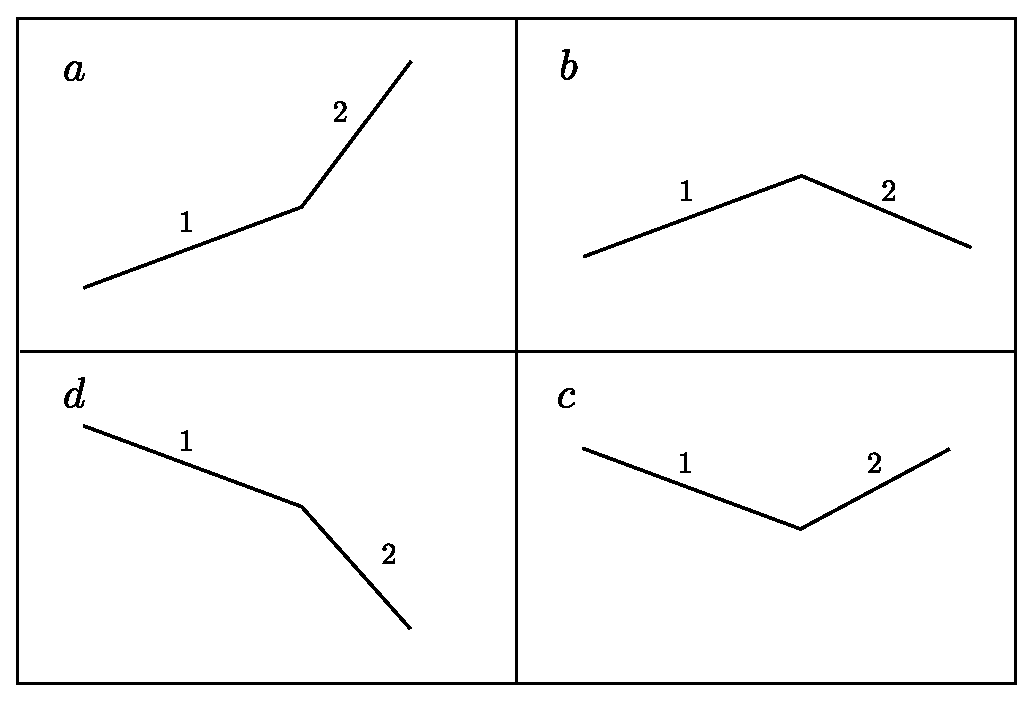
\includegraphics[width=\textwidth]{Rysunek0_all2.eps}
 \caption{Symbolic quadrant of response (second line) for market movement (first line)}
\end{figure}
\FloatBarrier



In this quadrant in quarters a) and b) we have situations (2) and (3) - ie, the closing value of the i bar $C_i$ is greater than the average of the last m bars. The first line in those quarters is addressed to top - market is on the rise. In the quarter, a) reaction to the growth of the market is to open a long position (2). The investor behaves as if he was convinced of the existence of a growing trend. In the quarter b) investors react on market growth with opening the short position. The investor behaves as if he predicts horizontal trend.

Conversely in quarters, c) and d) the first movement of the market is declining and investor reaction is recorded appropriately in decisions (4) and (5). In quarter c) investor behaves as if he predicts horizontal trend and opens long position (4) and in quarter d) beliving of drawdown trend he opens short position (5). \\
These situations are both shown in Figure 2\\
\begin{figure}[h]
\centering
\centering 
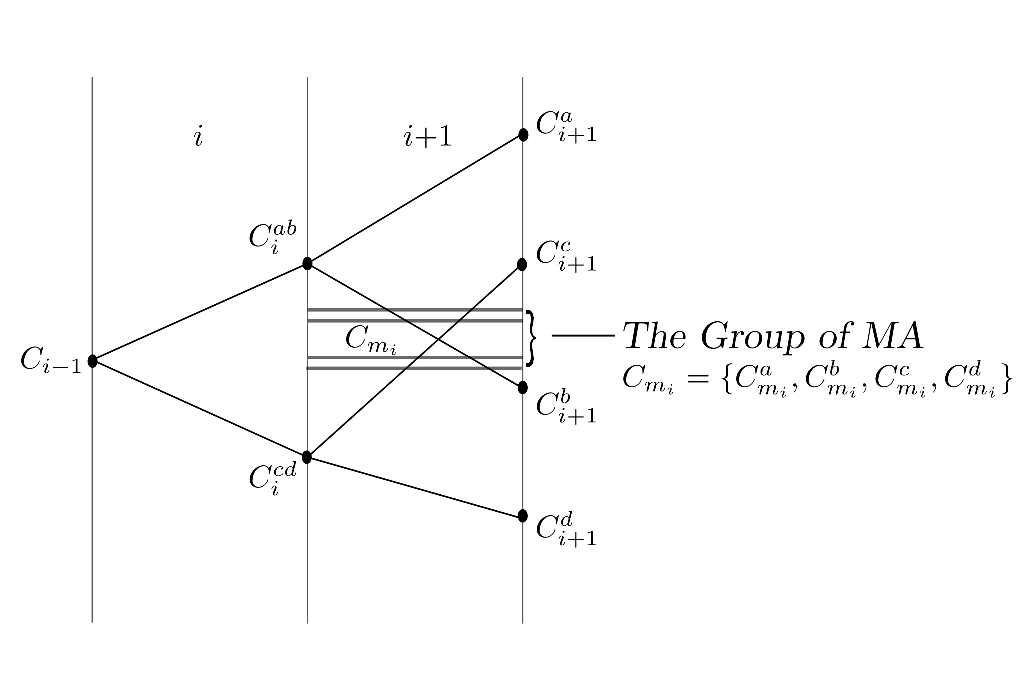
\includegraphics[width=\textwidth]{rysunek1pp.eps}
\caption{All possible situations for four different moving averages}
\end{figure}
\FloatBarrier
\indent Figure 2 shows the situation at the close of $(i-1)$th bar marked as $C_{i-1}$. The investor is following the situation in the i-th bar and at the moment of its close may immediately calculate each of the four average (1). Depending on the direction in which market has changed (upwards or downwards) we are dealing with quarters $a$ and $b$ of quadrant (If there is a price growth of the observed asset) or quarters $c$ and $d$ if there is a decrease.
Because, at the moment of end of the i bar it can be calculated  value of each of the four averages it can also be checked, if some of opening conditions (2)-(5) are passed. These four situations extracted from Figure 2 are shown in Figure 3, where in turn are explained  decision-making situations for the four quarters quadrant (Fig. 1)\\
\begin{figure}[h]
\centering
\begin{minipage}{.49\linewidth}
\centering 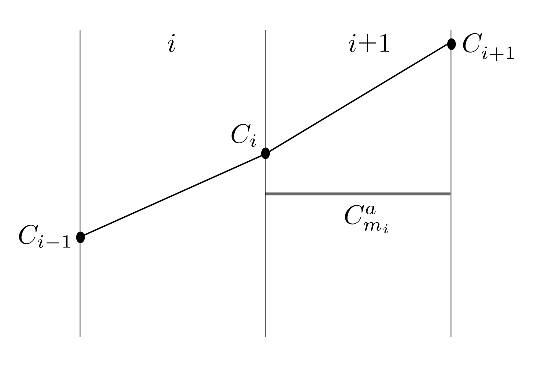
\includegraphics[width=\textwidth]{rysunek2a.eps}
\subcaption{Version a}
\label{jedno}
\end{minipage}
\begin{minipage}{.49\linewidth}
\centering 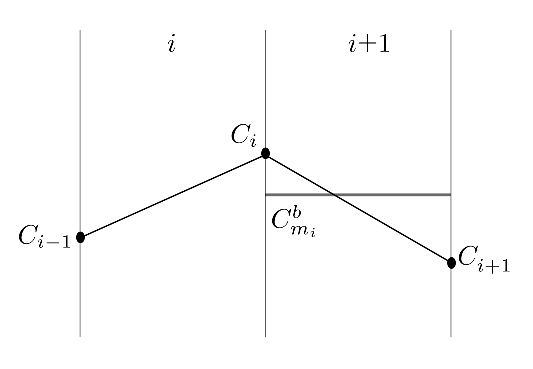
\includegraphics[width=\textwidth]{rysunek2b.eps}
\subcaption{Version b}
\label{dwu}
\end{minipage}
\\
\begin{minipage}{.49\linewidth}
\centering 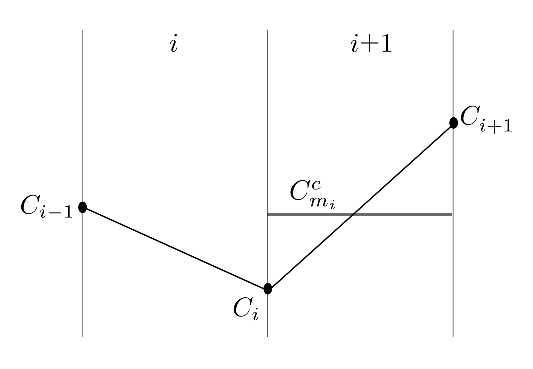
\includegraphics[width=\textwidth]{rysunek2c.eps}
\subcaption{Version c}
\label{cztero}
\end{minipage}
\begin{minipage}{.49\linewidth}
\centering 
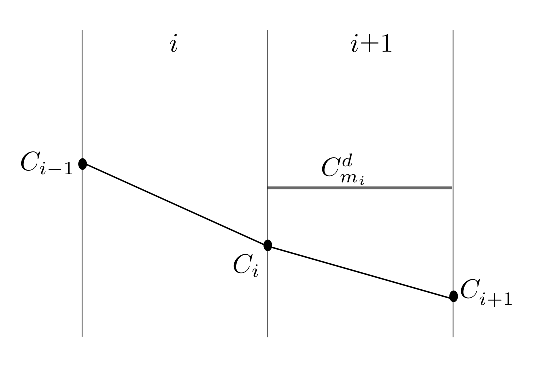
\includegraphics[width=\textwidth]{rysunek2d.eps}
\subcaption{Version d}
\label{mansard}
\end{minipage}
\caption{Separate strategies}
\end{figure}
\FloatBarrier
\indent The following sketches from a) to d) shows the change in the market against a particular average from $C^d_{m_{i}}$ to $C^a_{m_{i}}$.\\
\indent Each of these averages is counted step by step (bar) separately for each of the four situations, and of course the condition to open a position associated with a particular situation may occur or not. For example, if the closing value of the i-th bar in the situation a) will be below $C^a_{m_{i}}$ then opening long position won't occur.\\
\indent Extremely important in this strategy is the one and only parameter - number of last bar closures for average calculation. In each quarter of quadrant, in the general case the number is different. It is determined for a dedicated n number of bars, acting learner section of the time series so that for example for quarter a) :\\
\begin{equation}
	m_a = argmax (\sum y_i  )
\end{equation}
where: $yi = C_{i+1} - C_{i}$ for i=1, ..., n and complying  condition (2).\\
\indent So $m_{a}$ is the parameter learned on a particular section of a time series. This m value,for which achieves a maximum gain of opened positions (for quarter a) long). On another length of time series, by (6) it could have different value. Similarly, for the parameters $m_{b}$, $m_{c}$ and $m_{d}$.\\
\indent Use of this strategy makes the investor no longer think about the market in the traditional way trying to recognize what kind of a trend at the moment there is or whether this trend has just changed. Machine that is learned the optimal value of m for each quarter of quadrant takes over this role and makes decisions in every of four possible investment situations. Take these decisions only when each of four calculated optimal moving averages condition is satisfied to open specific position.
These strategy has been tested on the following markets as simple as possible. When was satisfied, one or more of the opening conditions (2) – (5) then position has been opened and closed at the close of the $(i +1)$th bar.





\section{The test results}
\indent The charts below show the curves of capital accumulation for each quarter of quadrant. Each graph represents one decision-making situation with the best parameter, number of last closures to calculate moving average. Fifth diagram shows the (S1s) cumulative strategy value. Which is the sum of profit of all open positions at this moment. Obviously all component strategies are calculated for the best parameter for each one of them.\\
\indent Following tables present the results of conducted simulations aimed at finding the best number of bars required to calculate means (bestMALength). Column "strategy" specifies which strategy was used, "profit" - the cumulative sum of the profit. Third column, "bestCalmar", represents Calmar Ratio which describes profit-to-maximum drawdown ratio. Low Calmar Ratio indicates poor investment performance on a risk-adjusted basis during certain time span. Last column "la" presents the number of open positions.
The study of strategy was carried out on the following markets:
\begin{itemize}
\item currency pairs: EURJPY, USDJPY, GBPUSD, EURUSD,
\item indices: FUS500, BOSSAPLN,
\item commodities: FGOLD. FSILVER.
\end{itemize}
BOSSAPLN is currency index that represents ratio of PLN to four other currencies. Every currency pair used to calculate index has other weight USDPLN (40\%), EURPLN (50\%), GBPPLN (5\%), CHFPLN (5\%).
\newpage
\begin{table}[!t]
\caption{Profits for all strategy quadrants for EURJPY} 
 \begin{center} 
 \begin{tabular}{|l|l|l|l|l|} 
 \hline \textbf{strategy} & \textbf{profit} & \textbf{bestCalmar} & \textbf{bestMALength} & \textbf{la} \\ \hline  
S1a & 26.18 & 5.59 & 24 & 2764\\ \hline 
S1b & -14.77 & -0.67 & 6 & 2660\\ \hline 
S1c & 15.74 & 2.49 & 6 & 2332\\ \hline 
S1d & -4.57 & -0.47 & 21 & 2226\\ \hline 
S1s & 22.54 & 3.25 & Group of MA & 4975\\ 
\hline \end{tabular} 
 \end{center} 
 \end{table}
\FloatBarrier

\begin{figure}[h]
\centering
\begin{minipage}{.49\linewidth}
\centering 
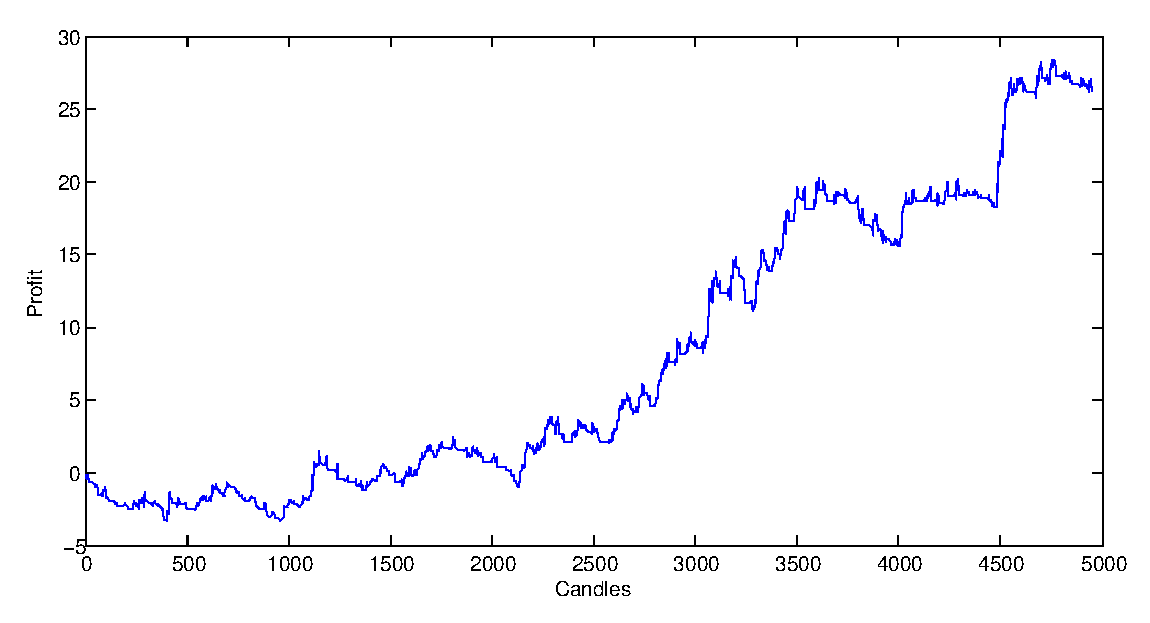
\includegraphics[width=0.82\textwidth]{images/S1a_eurjpy.eps}
\subcaption{Profit - S1a}
\label{jedno}
\end{minipage}
\begin{minipage}{.49\linewidth}
\centering 
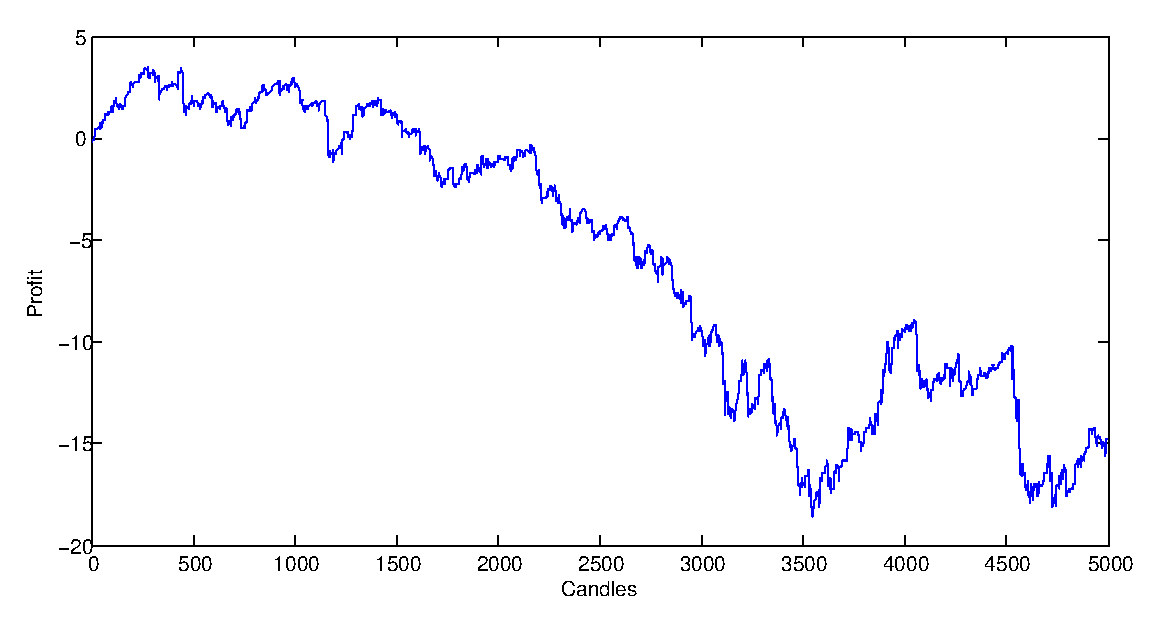
\includegraphics[width=0.82\textwidth]{images/S1b_eurjpy.eps}
\subcaption{Profit - S1b}
\label{dwu}
\end{minipage}
\\
\begin{minipage}{.49\linewidth}
\centering 
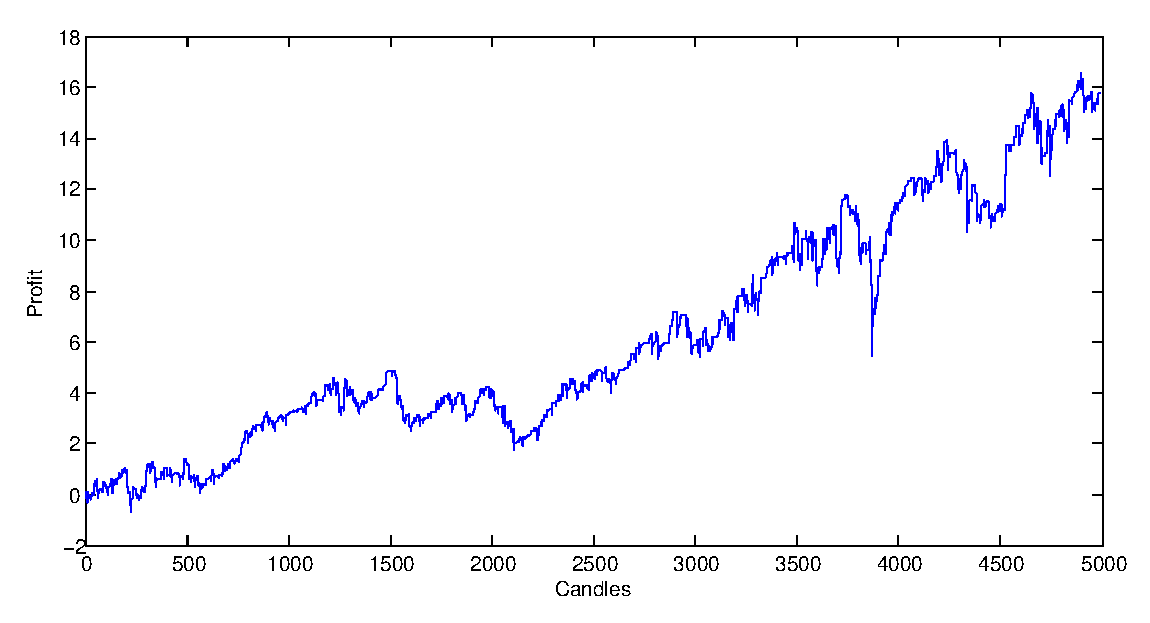
\includegraphics[width=0.82\textwidth]{images/S1c_eurjpy.eps}
\subcaption{Profit- S1c}
\label{cztero}
\end{minipage}
\begin{minipage}{.49\linewidth}
\centering 
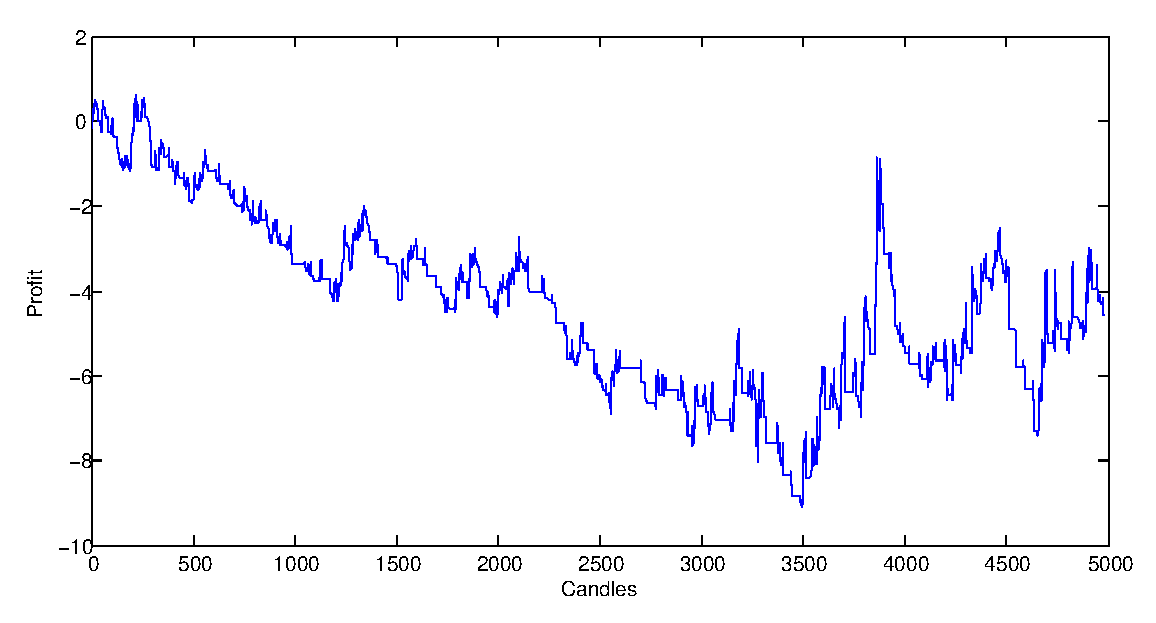
\includegraphics[width=0.82\textwidth]{images/S1d_eurjpy.eps}
\subcaption{Profit - S1d}
\label{mansard}
\end{minipage}
\begin{minipage}{\linewidth}
\centering 
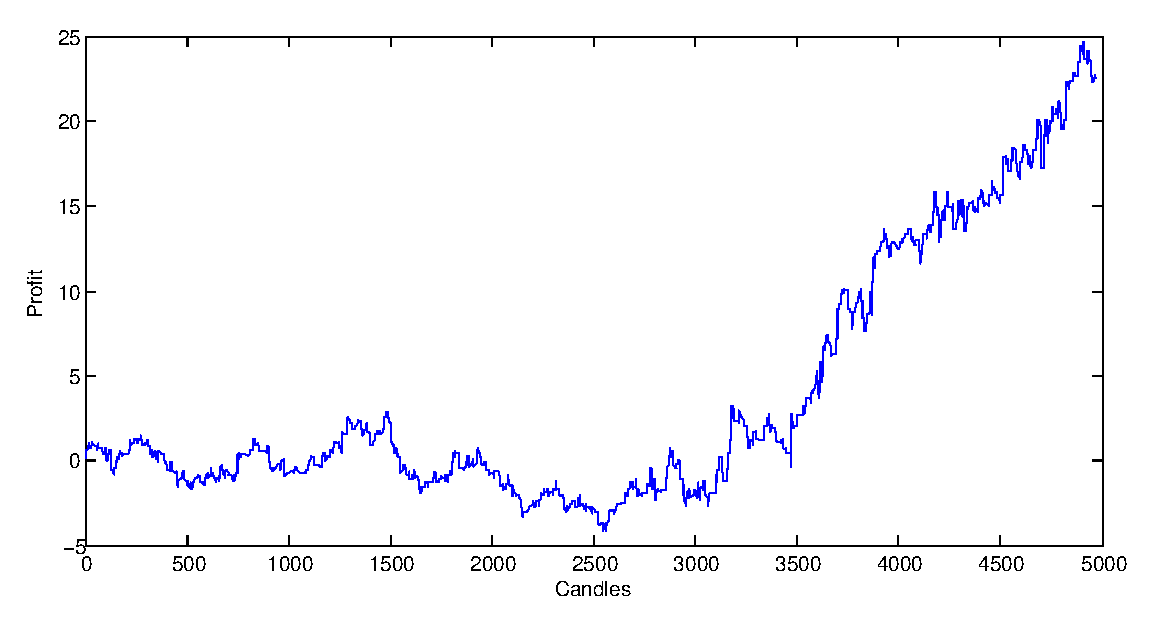
\includegraphics[width=0.6\textwidth]{images/S1s_eurjpy.eps}
\label{mansard}
\subcaption{Profit - S1s}
\end{minipage}
\caption{EURJPY market results}
\end{figure}
\FloatBarrier
%%%%%%%%%%%%%%%%%%%%%%%%%%%%%%%%
\newpage
\begin{table}[!t]
\caption{Profits for all strategy quadrants for USDJPY} 
 \begin{center} 
 \begin{tabular}{|l|l|l|l|l|} 
 \hline \textbf{strategy} & \textbf{profit} & \textbf{bestCalmar} & \textbf{bestMALength} & \textbf{la} \\ \hline  
S1a & 17.19 & 8.24 & 18 & 2693\\ \hline 
S1b & -9.80 & -0.74 & 54 & 2665\\ \hline 
S1c & 5.65 & 2.06 & 54 & 2280\\ \hline 
S1d & 1.87 & 0.61 & 18 & 2287\\ \hline 
S1s & 14.85 & 5.68 & Group of MA & 4945\\ 
\hline \end{tabular} 
 \end{center} 
 \end{table}
\FloatBarrier

\begin{figure}[h]
\centering
\begin{minipage}{.49\linewidth}
\centering 
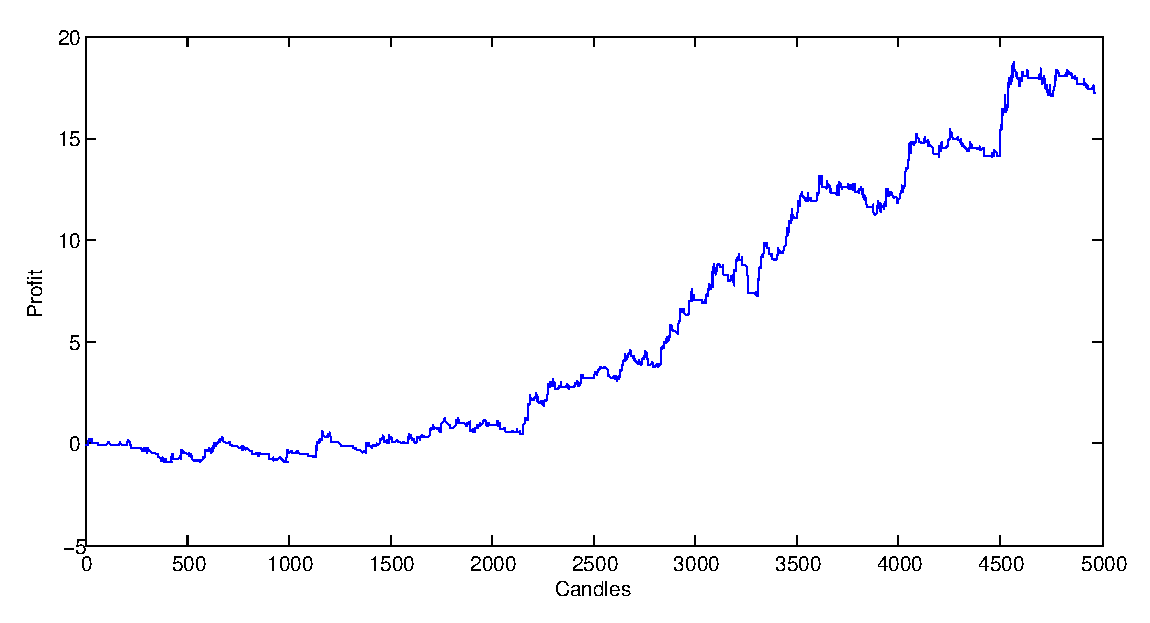
\includegraphics[width=0.82\textwidth]{images/S1a_usdjpy.eps}
\subcaption{Profit - S1a}
\label{jedno}
\end{minipage}
\begin{minipage}{.49\linewidth}
\centering 
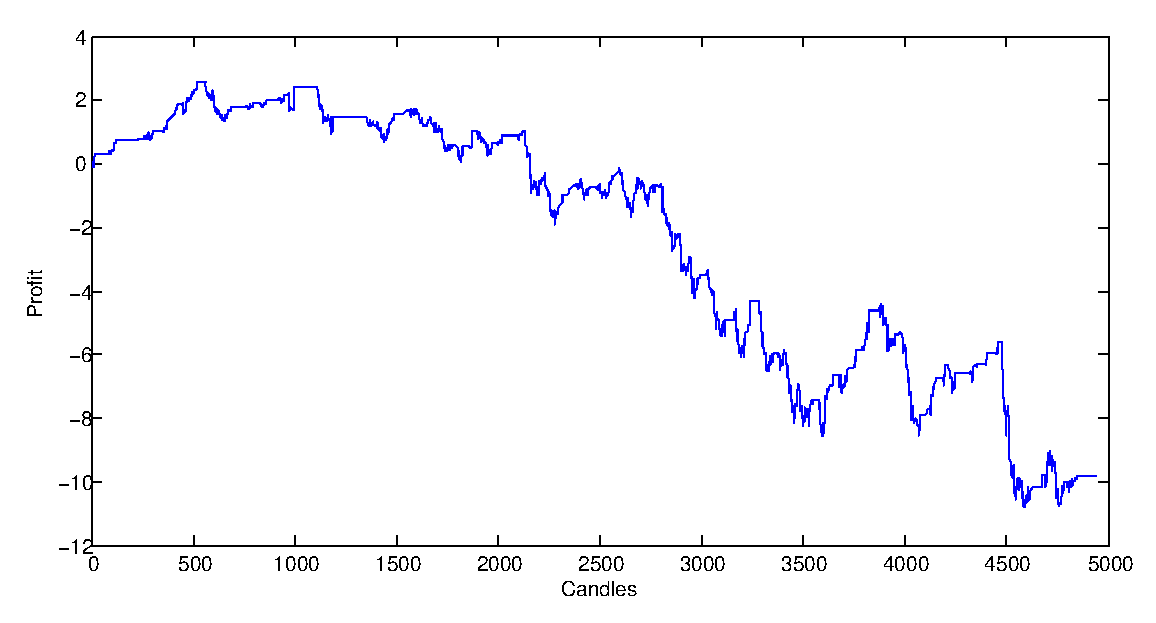
\includegraphics[width=0.82\textwidth]{images/S1b_usdjpy.eps}
\subcaption{Profit - S1b}
\label{dwu}
\end{minipage}
\\
\begin{minipage}{.49\linewidth}
\centering 
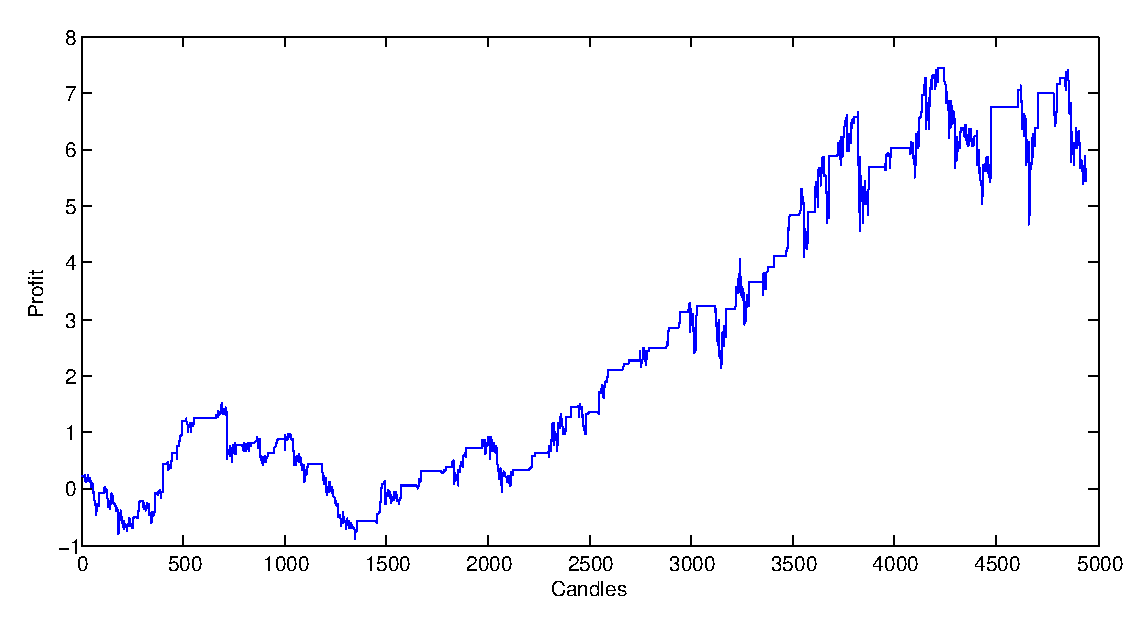
\includegraphics[width=0.82\textwidth]{images/S1c_usdjpy.eps}
\subcaption{Profit- S1c}
\label{cztero}
\end{minipage}
\begin{minipage}{.49\linewidth}
\centering 
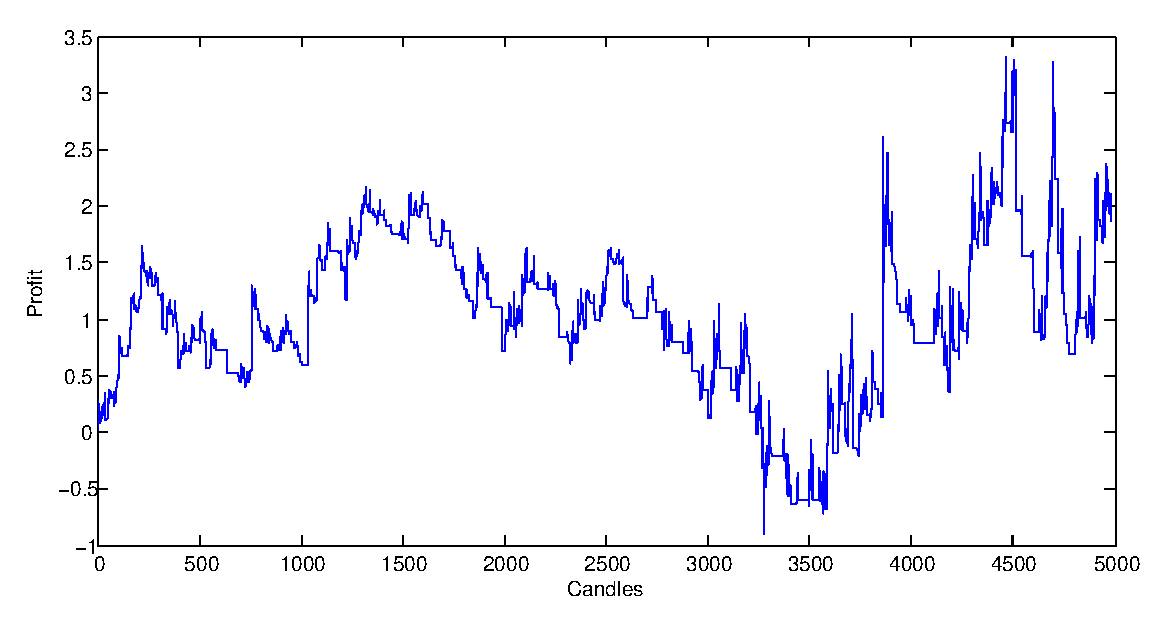
\includegraphics[width=0.82\textwidth]{images/S1d_usdjpy.eps}
\subcaption{Profit - S1d}
\label{mansard}
\end{minipage}
\begin{minipage}{\linewidth}
\centering 
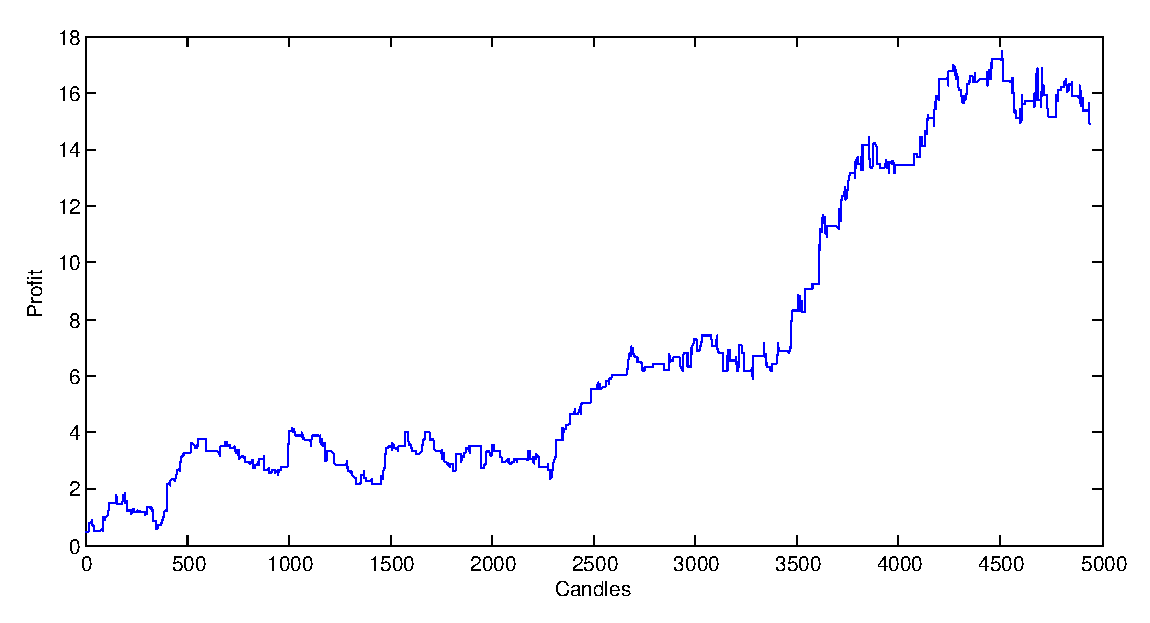
\includegraphics[width=0.6\textwidth]{images/S1s_usdjpy.eps}
\label{mansard}
\subcaption{Profit - S1s}
\end{minipage}
\caption{USDJPY market results}
\end{figure}
\FloatBarrier


%%%%%%%%%%%%%%%%%%%%%%%%%%%%%%%%
\newpage
\begin{table}[!t]
\caption{Profits for all strategy quadrants for GBPUSD} 
 \begin{center} 
 \begin{tabular}{|l|l|l|l|l|} 
 \hline \textbf{strategy} & \textbf{profit} & \textbf{bestCalmar} & \textbf{bestMALength} & \textbf{la} \\ \hline  
S1a & 0.06 & 1.06 & 92 & 2588\\ \hline 
S1b & 0.12 & 3.41 & 5 & 2513\\ \hline 
S1c & 0.15 & 3.11 & 5 & 2475\\ \hline 
S1d & 0.02 & 0.31 & 92 & 2319\\ \hline 
S1s & 0.36 & 6.89 & Group of MA & 4907\\ 
\hline \end{tabular} 
 \end{center} 
 \end{table}
\FloatBarrier

\begin{figure}[h]
\centering
\begin{minipage}{.49\linewidth}
\centering 
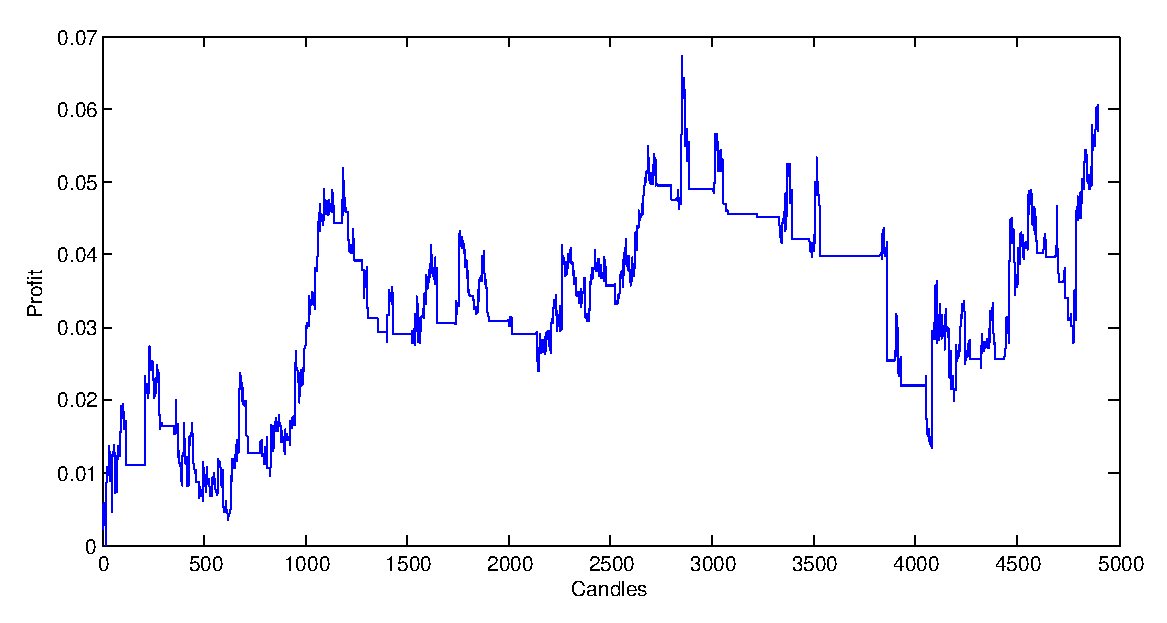
\includegraphics[width=0.82\textwidth]{images/S1a_gbpusd.eps}
\subcaption{Profit - S1a}
\label{jedno}
\end{minipage}
\begin{minipage}{.49\linewidth}
\centering 
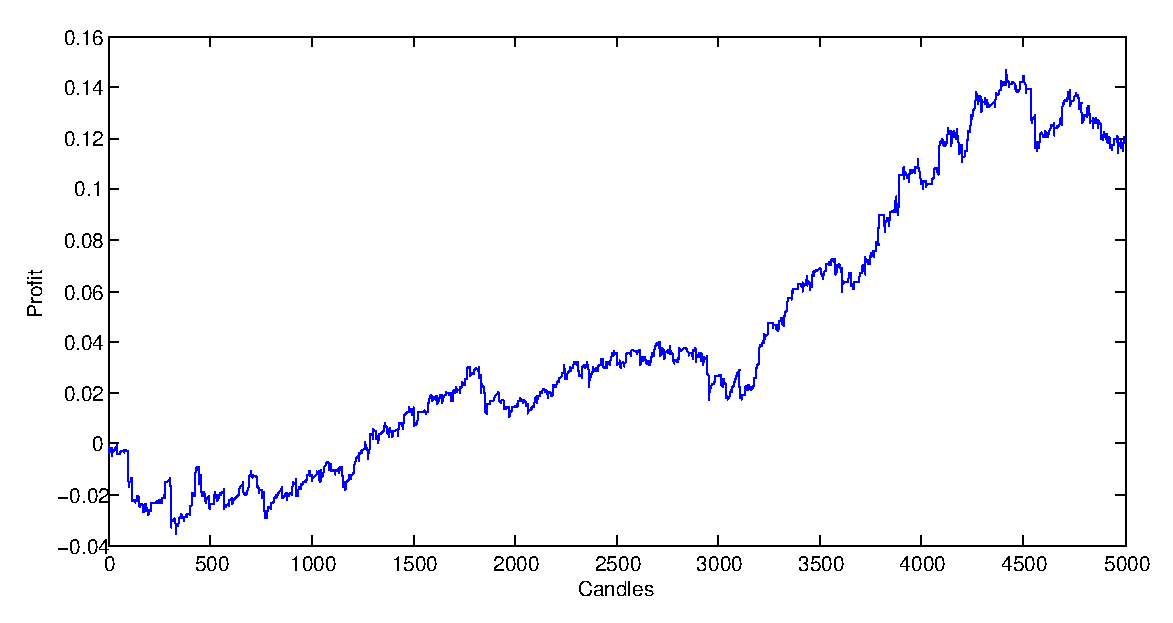
\includegraphics[width=0.82\textwidth]{images/S1b_gbpusd.eps}
\subcaption{Profit - S1b}
\label{dwu}
\end{minipage}
\\
\begin{minipage}{.49\linewidth}
\centering 
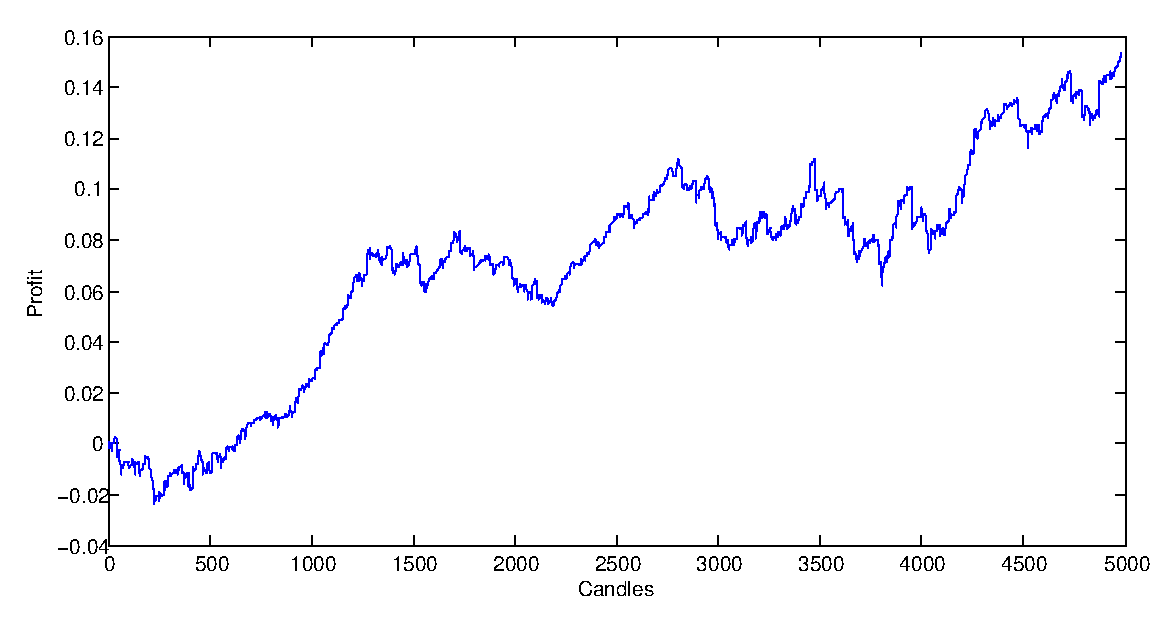
\includegraphics[width=0.82\textwidth]{images/S1c_gbpusd.eps}
\subcaption{Profit- S1c}
\label{cztero}
\end{minipage}
\begin{minipage}{.49\linewidth}
\centering 
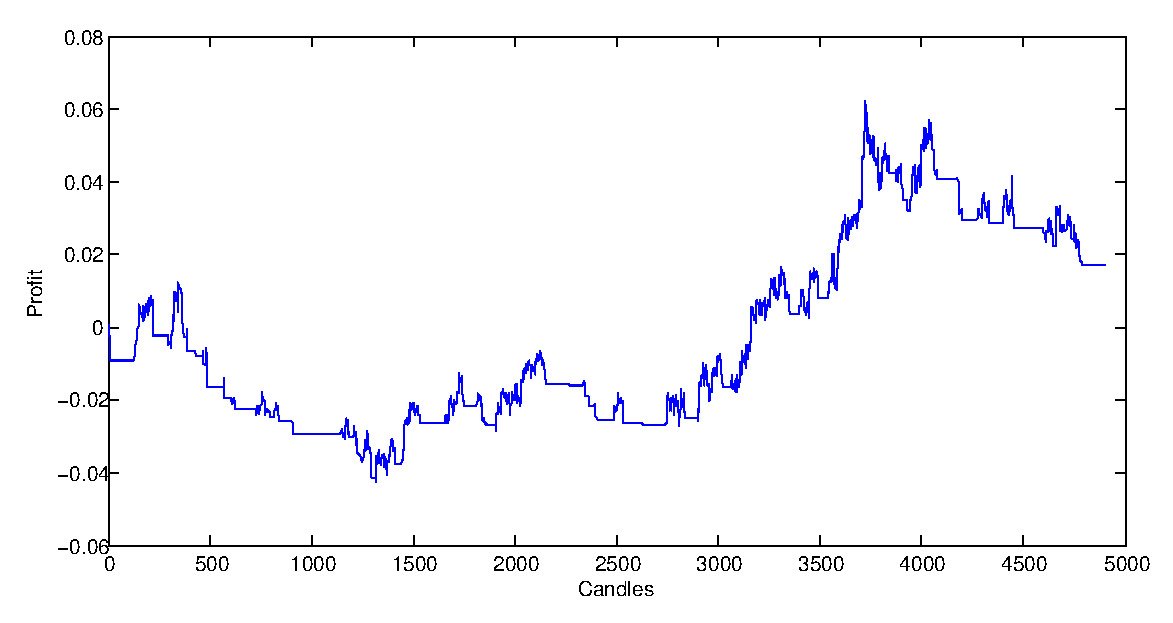
\includegraphics[width=0.82\textwidth]{images/S1d_gbpusd.eps}
\subcaption{Profit - S1d}
\label{mansard}
\end{minipage}
\begin{minipage}{\linewidth}
\centering 
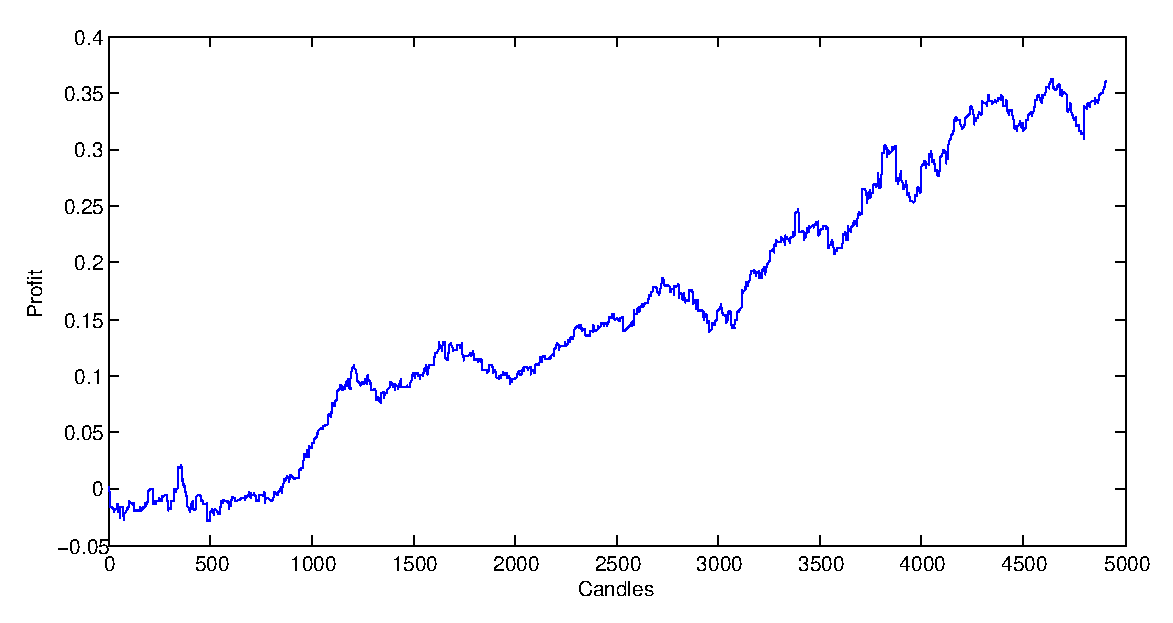
\includegraphics[width=0.6\textwidth]{images/S1s_gbpusd.eps}
\label{mansard}
\subcaption{Profit - S1s}
\end{minipage}
\caption{GBPUSD market results}
\end{figure}
\FloatBarrier

%%%%%%%%%%%%%%%%%%%%%%%%%%%%%%%%
\newpage
\begin{table}[!t]
\caption{Profits for all strategy quadrants for EURUSD} 
 \begin{center} 
 \begin{tabular}{|l|l|l|l|l|} 
 \hline \textbf{strategy} & \textbf{profit} & \textbf{bestCalmar} & \textbf{bestMALength} & \textbf{la} \\ \hline  
S1a & 0.09 & 1.84 & 33 & 2635\\ \hline 
S1b & 0.01 & 0.16 & 5 & 2587\\ \hline 
S1c & 0.12 & 3.45 & 5 & 2406\\ \hline 
S1d & -0.02 & -0.49 & 33 & 2331\\ \hline 
S1s & 0.21 & 3.31 & Group of MA & 4966\\ 
\hline \end{tabular} 
 \end{center} 
 \end{table}
\FloatBarrier

\begin{figure}[h]
\centering
\begin{minipage}{.49\linewidth}
\centering 
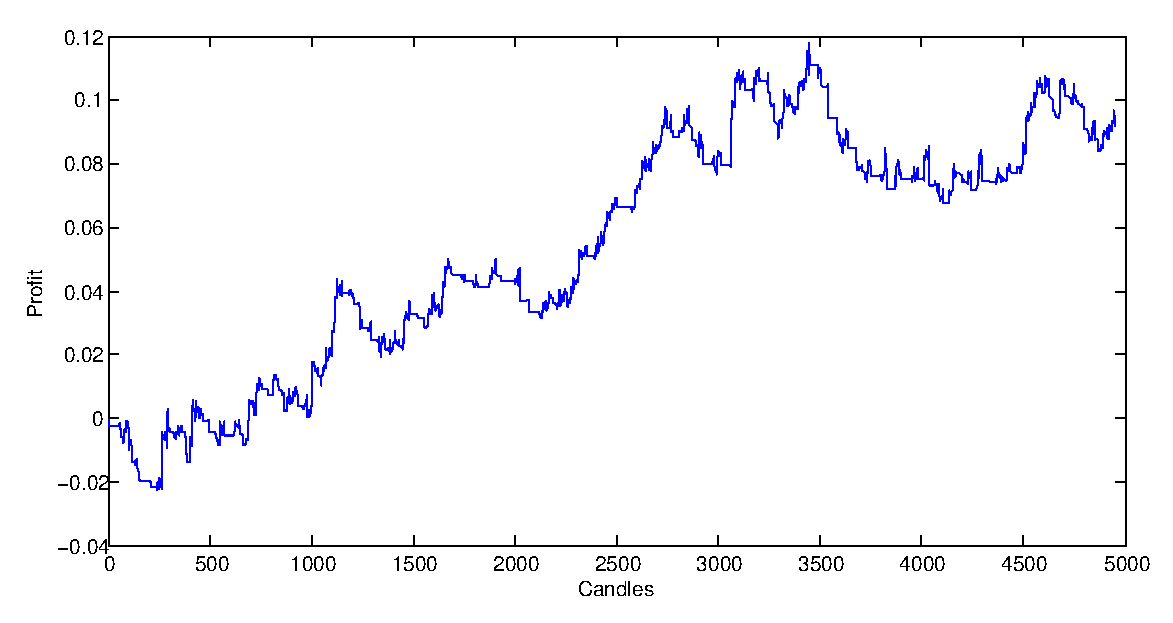
\includegraphics[width=0.82\textwidth]{images/S1a_eurusd.eps}
\subcaption{Profit - S1a}
\label{jedno}
\end{minipage}
\begin{minipage}{.49\linewidth}
\centering 
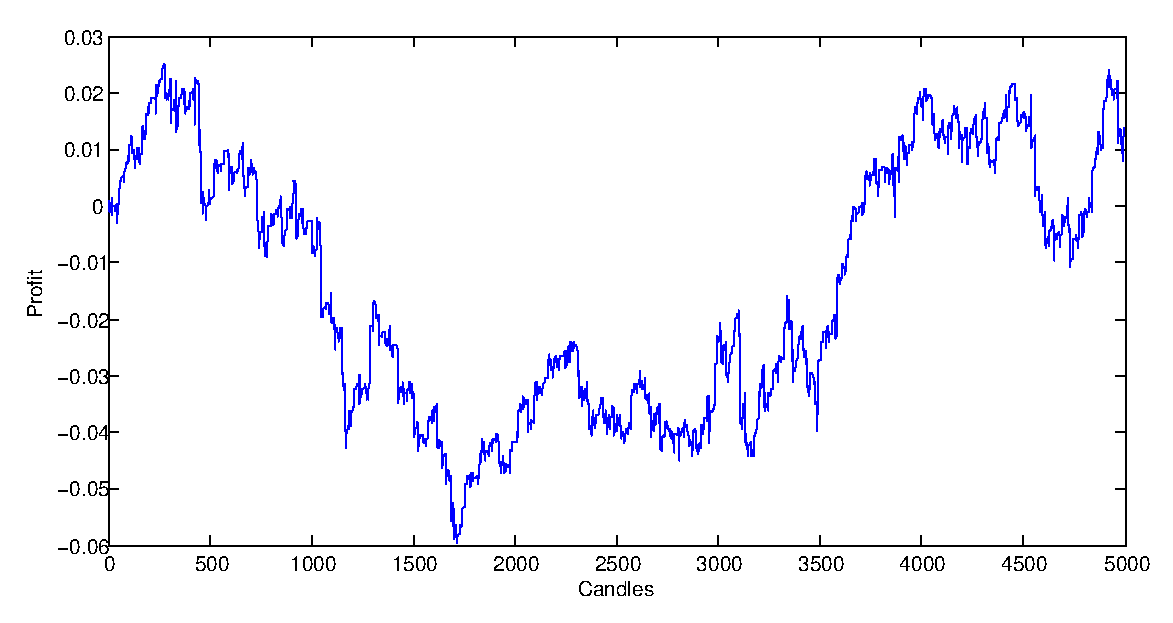
\includegraphics[width=0.82\textwidth]{images/S1b_eurusd.eps}
\subcaption{Profit - S1b}
\label{dwu}
\end{minipage}
\\
\begin{minipage}{.49\linewidth}
\centering 
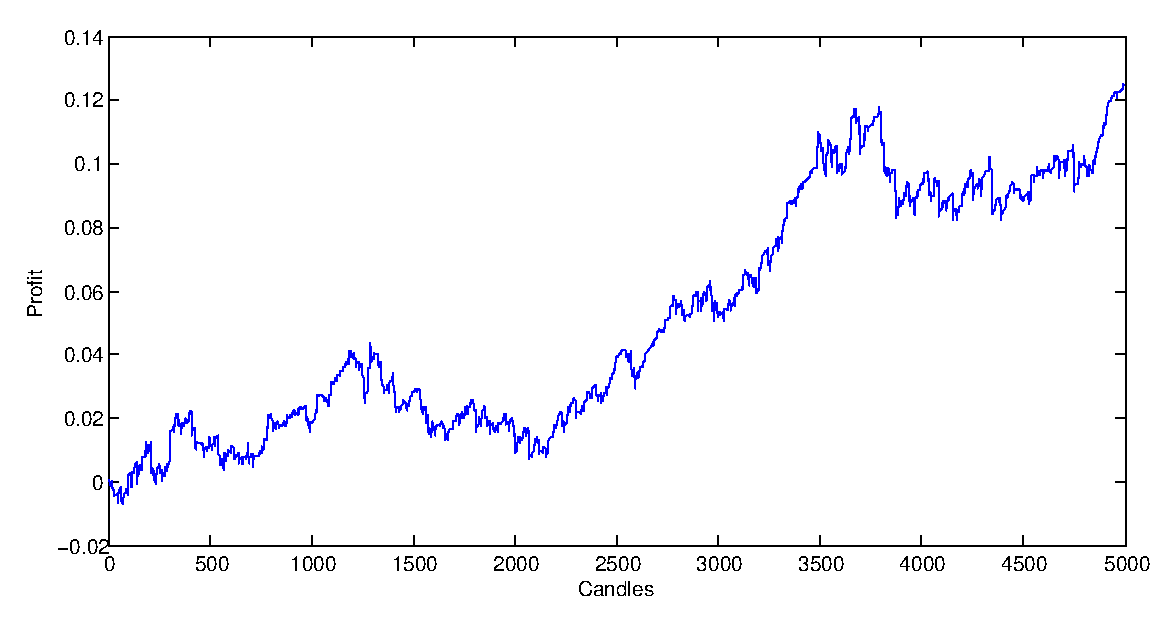
\includegraphics[width=0.82\textwidth]{images/S1c_eurusd.eps}
\subcaption{Profit- S1c}
\label{cztero}
\end{minipage}
\begin{minipage}{.49\linewidth}
\centering 
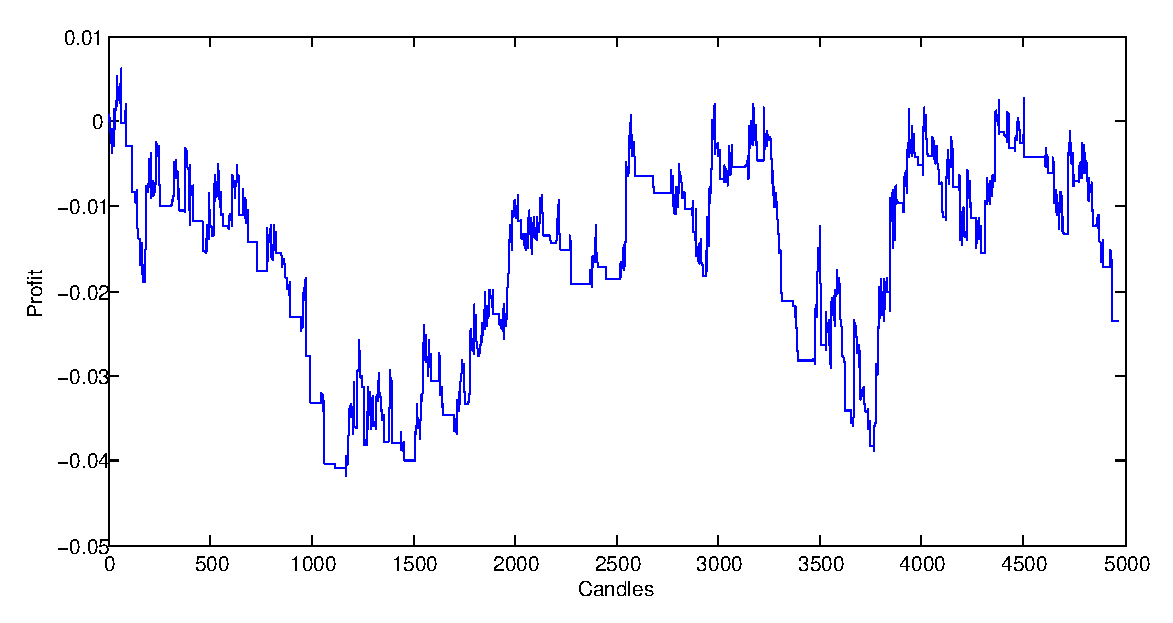
\includegraphics[width=0.82\textwidth]{images/S1d_eurusd.eps}
\subcaption{Profit - S1d}
\label{mansard}
\end{minipage}
\begin{minipage}{\linewidth}
\centering 
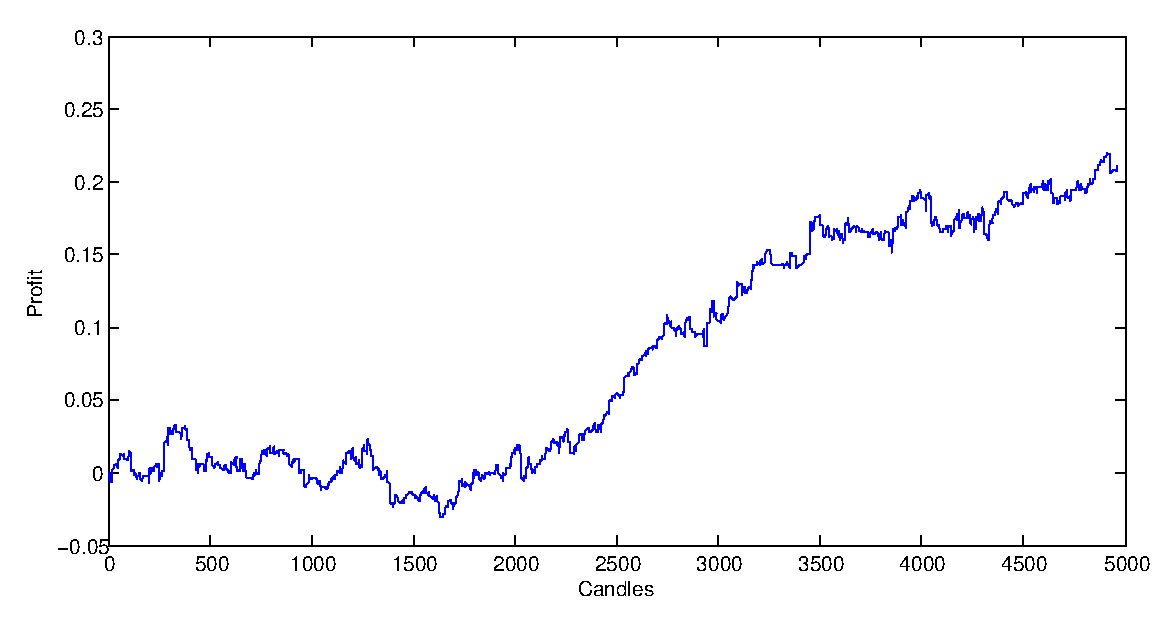
\includegraphics[width=0.6\textwidth]{images/S1s_eurusd.eps}
\label{mansard}
\subcaption{Profit - S1s}
\end{minipage}
\caption{EURUSD market results}
\end{figure}
\FloatBarrier


%%%%%%%%%%%%%%%%%%%%%%%%%%%%%%%%


%%%%%%%%%%%%%%%%%%%%%%%%%%%%%%%%
\newpage
\begin{table}[!t]
\caption{Profits for all strategy quadrants for FUS500} 
 \begin{center} 
 \begin{tabular}{|l|l|l|l|l|} 
 \hline \textbf{strategy} & \textbf{profit} & \textbf{bestCalmar} & \textbf{bestMALength} & \textbf{la} \\ \hline  
S1a & 274.89 & 5.44 & 83 & 3200\\ \hline 
S1b & -70.94 & -0.47 & 15 & 2798\\ \hline 
S1c & 291.62 & 4.26 & 15 & 2186\\ \hline 
S1d & -106.67 & -0.73 & 82 & 1723\\ \hline 
S1s & 344.29 & 2.08 & Group of MA & 4916\\ 
\hline \end{tabular} 
 \end{center} 
 \end{table}
\FloatBarrier

\begin{figure}[h]
\centering
\begin{minipage}{.49\linewidth}
\centering 
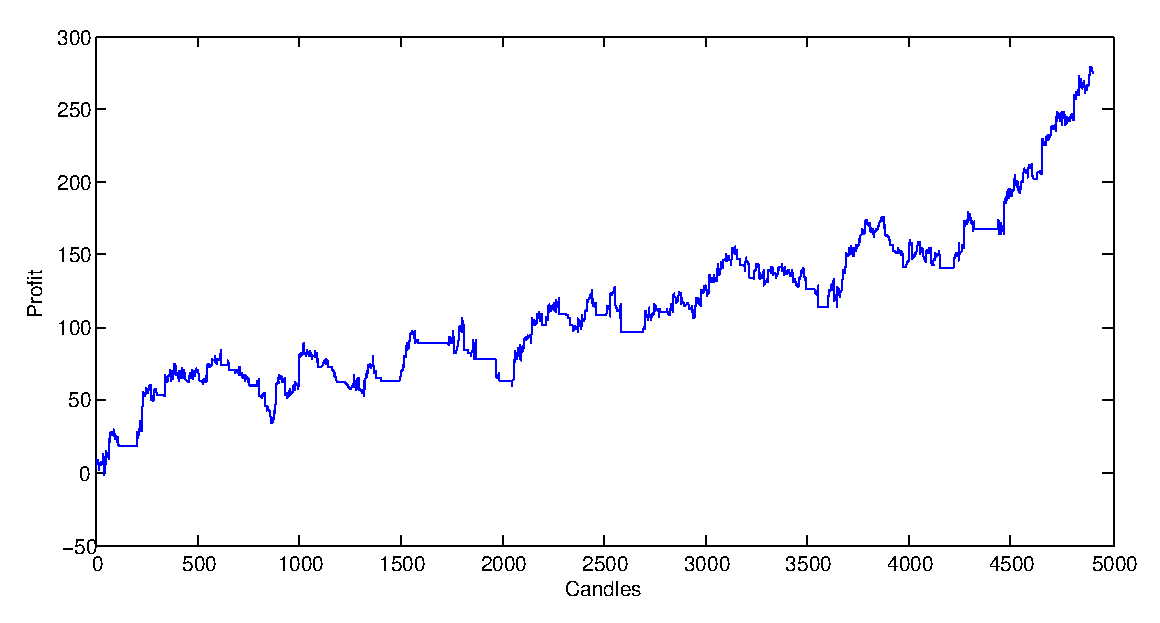
\includegraphics[width=0.82\textwidth]{images/S1a_fus.eps}
\subcaption{Profit - S1a}
\label{jedno}
\end{minipage}
\begin{minipage}{.49\linewidth}
\centering 
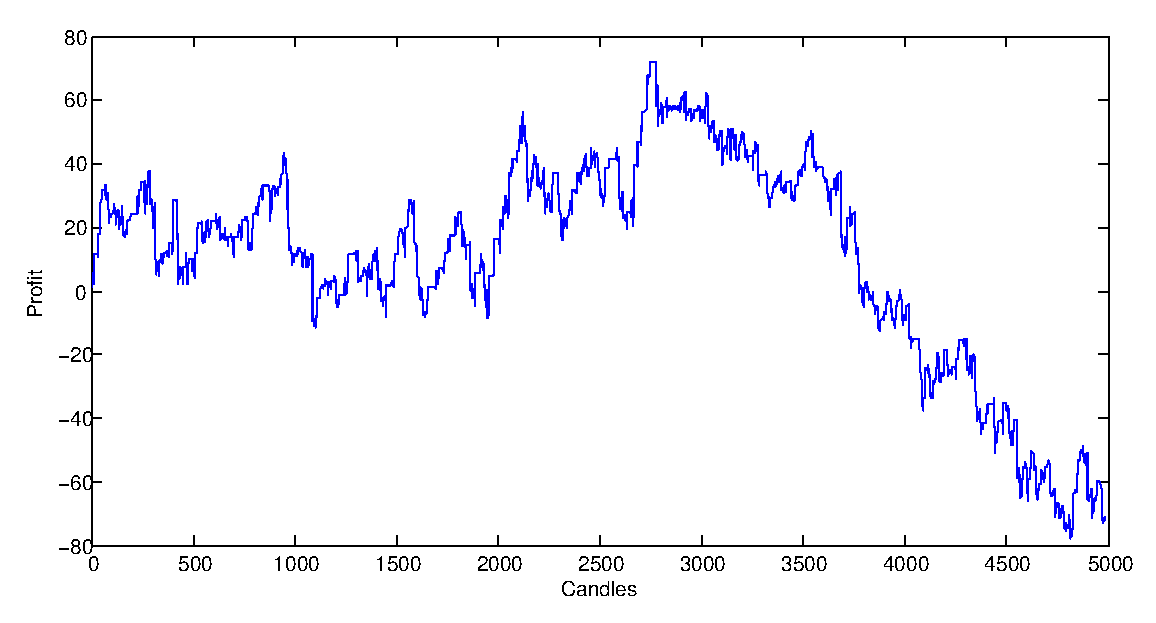
\includegraphics[width=0.82\textwidth]{images/S1b_fus.eps}
\subcaption{Profit - S1b}
\label{dwu}
\end{minipage}
\\
\begin{minipage}{.49\linewidth}
\centering 
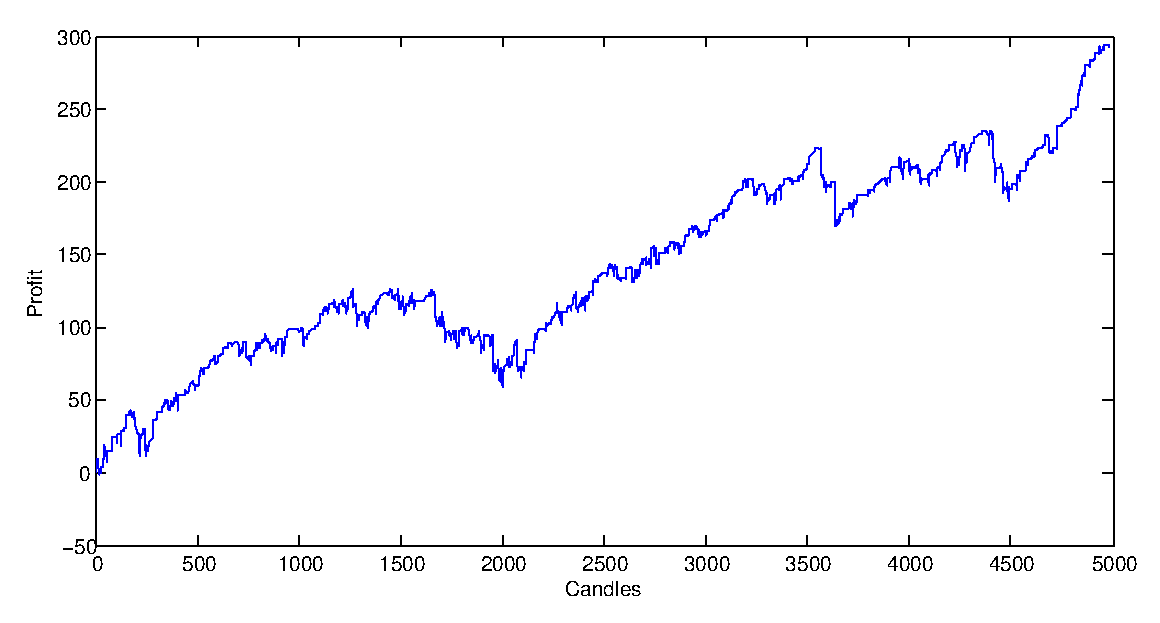
\includegraphics[width=0.82\textwidth]{images/S1c_fus.eps}
\subcaption{Profit- S1c}
\label{cztero}
\end{minipage}
\begin{minipage}{.49\linewidth}
\centering 
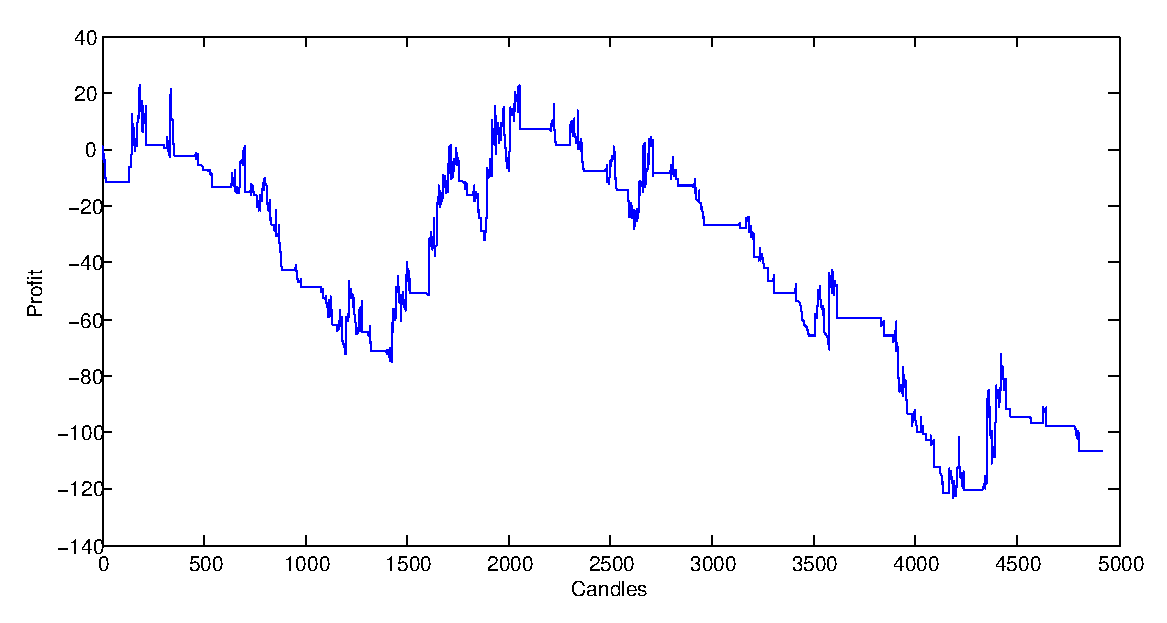
\includegraphics[width=0.82\textwidth]{images/S1d_fus.eps}
\subcaption{Profit - S1d}
\label{mansard}
\end{minipage}
\begin{minipage}{\linewidth}
\centering 
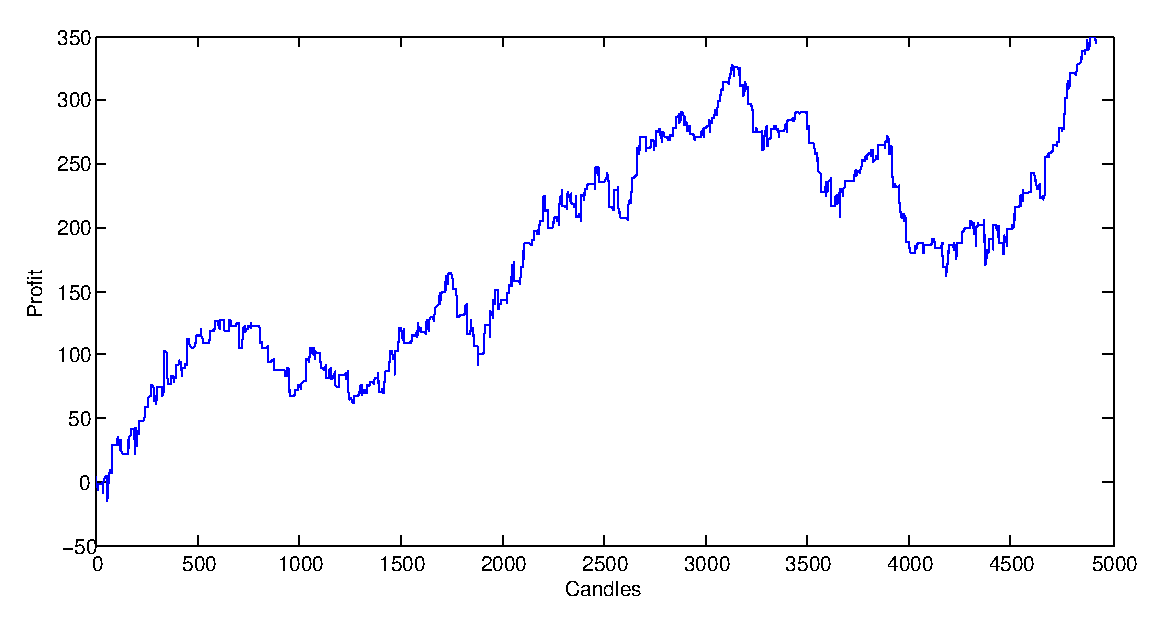
\includegraphics[width=0.6\textwidth]{images/S1s_fus.eps}
\label{mansard}
\subcaption{Profit - S1s}
\end{minipage}
\caption{FUS500 market results}
\end{figure}
\FloatBarrier


%%%%%%%%%%%%%%%%%%%%%%%%%%%%%%%%
\newpage
\begin{table}[!t]
\caption{Profits for all strategy quadrants for BOSSAPLN} 
 \begin{center} 
 \begin{tabular}{|l|l|l|l|l|} 
 \hline \textbf{strategy} & \textbf{profit} & \textbf{bestCalmar} & \textbf{bestMALength} & \textbf{la} \\ \hline  
S1a & 5.87 & 1.99 & 21 & 2474\\ \hline 
S1b & 2.86 & 0.61 & 5 & 2416\\ \hline 
S1c & 10.91 & 4.33 & 5 & 2547\\ \hline 
S1d & -2.23 & -0.42 & 21 & 2502\\ \hline 
S1s & 17.91 & 4.35 & Group of MA & 4978\\ 
\hline \end{tabular} 
 \end{center} 
 \end{table}
\FloatBarrier

\begin{figure}[h]
\centering
\begin{minipage}{.49\linewidth}
\centering 
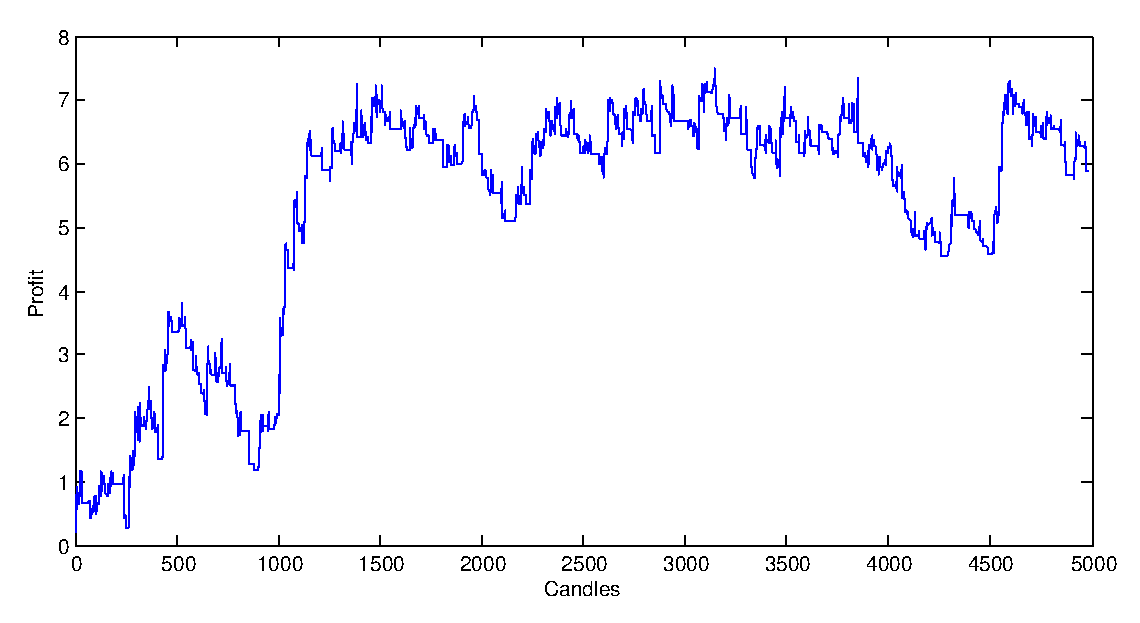
\includegraphics[width=0.82\textwidth]{images/S1a_bossa.eps}
\subcaption{Profit - S1a}
\label{jedno}
\end{minipage}
\begin{minipage}{.49\linewidth}
\centering 
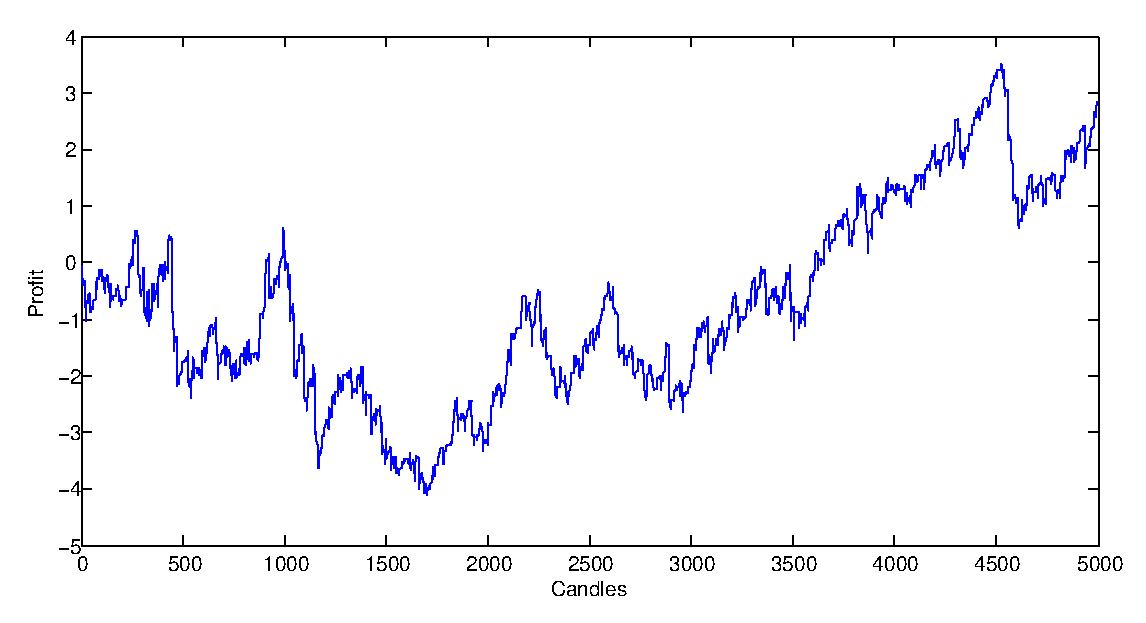
\includegraphics[width=0.82\textwidth]{images/S1b_bossa.eps}
\subcaption{Profit - S1b}
\label{dwu}
\end{minipage}
\\
\begin{minipage}{.49\linewidth}
\centering 
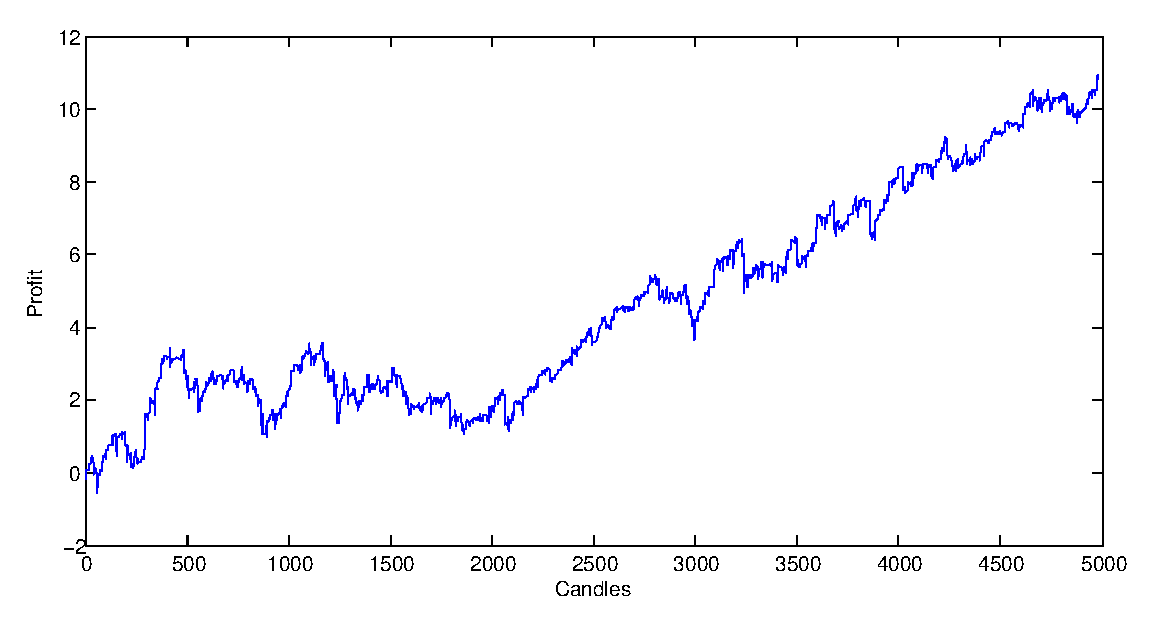
\includegraphics[width=0.82\textwidth]{images/S1c_bossa.eps}
\subcaption{Profit- S1c}
\label{cztero}
\end{minipage}
\begin{minipage}{.49\linewidth}
\centering 
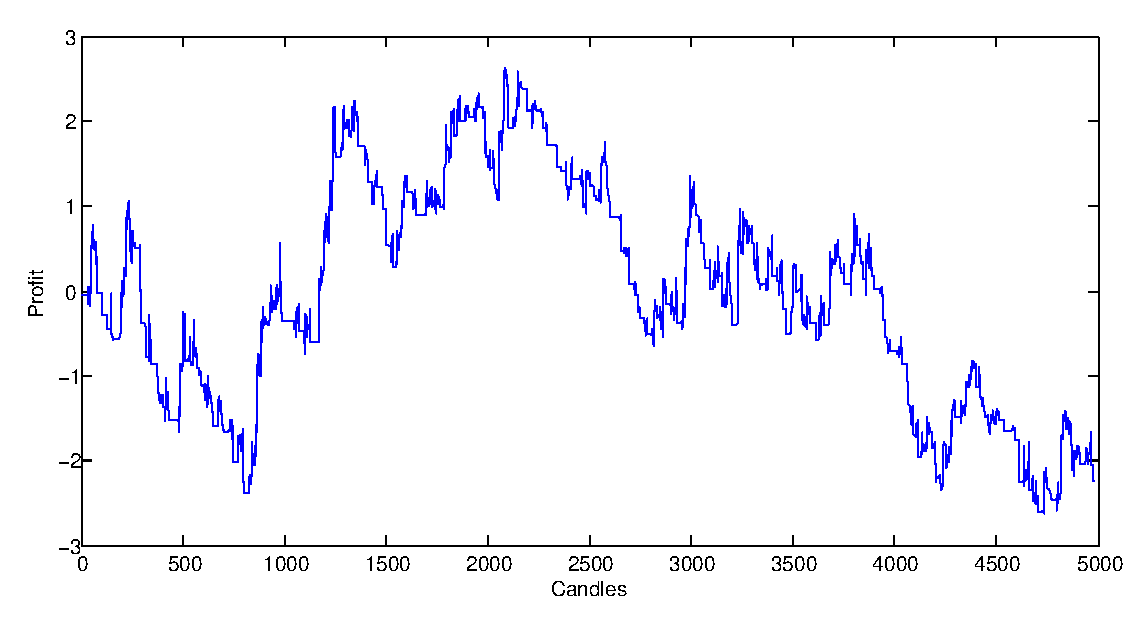
\includegraphics[width=0.82\textwidth]{images/S1d_bossa.eps}
\subcaption{Profit - S1d}
\label{mansard}
\end{minipage}
\begin{minipage}{\linewidth}
\centering 
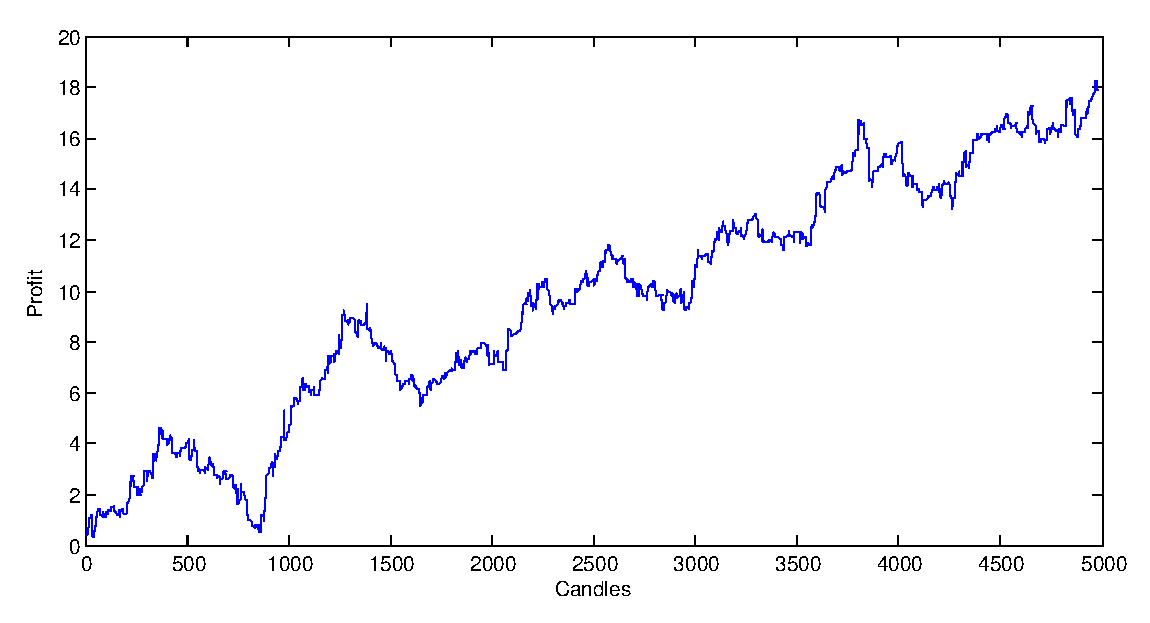
\includegraphics[width=0.6\textwidth]{images/S1s_bossa.eps}
\label{mansard}
\subcaption{Profit - S1s}
\end{minipage}
\caption{BOSSAPLN market results}
\end{figure}
\FloatBarrier




%%%%%%%%%%%%%%%%%%%%%%%%%%%%%%%%
\newpage
\begin{table}[!t]
\caption{Profits for all strategy quadrants for FGOLD} 
 \begin{center} 
 \begin{tabular}{|l|l|l|l|l|} 
 \hline \textbf{strategy} & \textbf{profit} & \textbf{bestCalmar} & \textbf{bestMALength} & \textbf{la} \\ \hline  
S1a & 61.16 & 0.59 & 51 & 2578\\ \hline 
S1b & 227.58 & 2.82 & 5 & 2519\\ \hline 
S1c & 30.38 & 0.12 & 5 & 2470\\ \hline 
S1d & 248.21 & 1.52 & 51 & 2370\\ \hline 
S1s & 599.88 & 4.60 & Group of MA & 4948\\ 
\hline \end{tabular} 
 \end{center} 
 \end{table}
\FloatBarrier

\begin{figure}[h]
\centering
\begin{minipage}{.49\linewidth}
\centering 
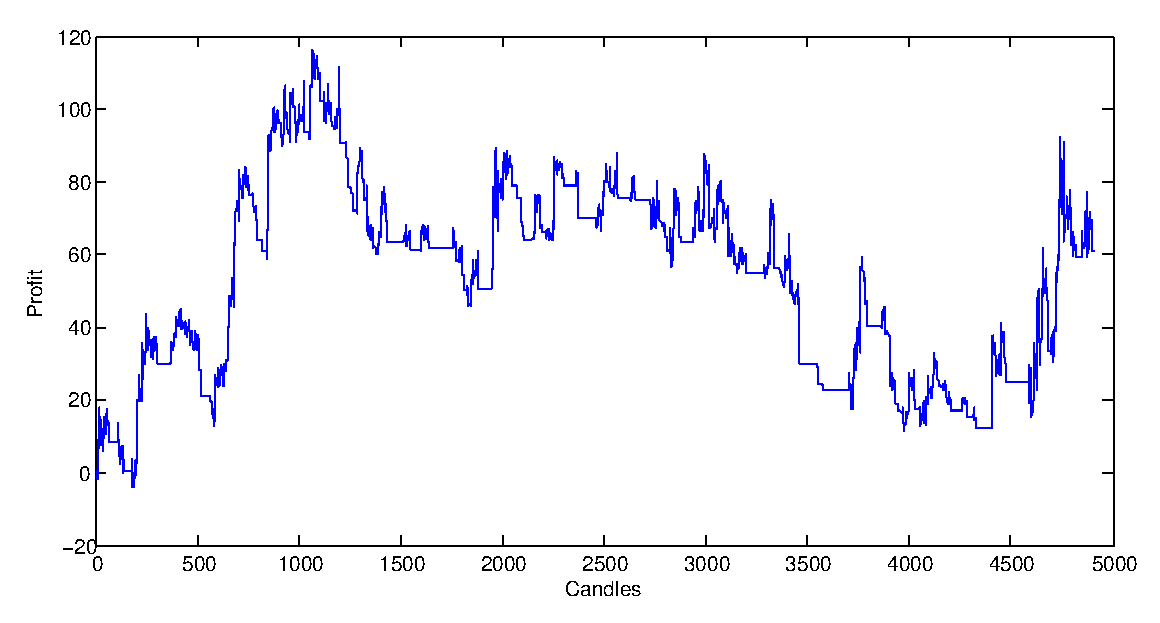
\includegraphics[width=0.82\textwidth]{images/S1a_gold.eps}
\subcaption{Profit - S1a}
\label{jedno}
\end{minipage}
\begin{minipage}{.49\linewidth}
\centering 
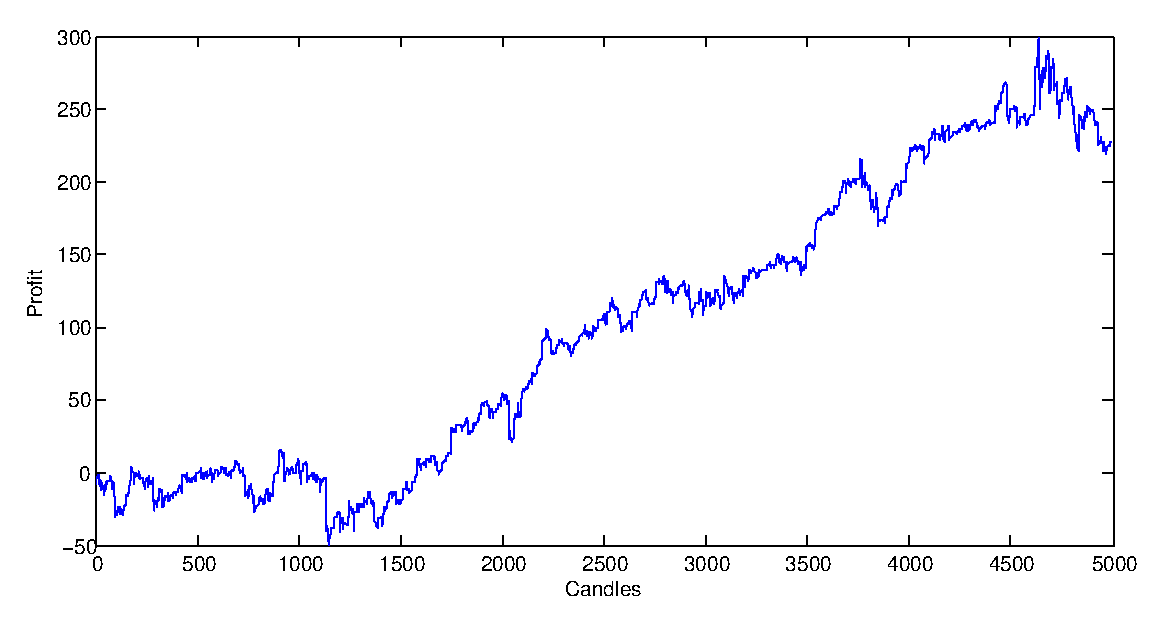
\includegraphics[width=0.82\textwidth]{images/S1b_gold.eps}
\subcaption{Profit - S1b}
\label{dwu}
\end{minipage}
\\
\begin{minipage}{.49\linewidth}
\centering 
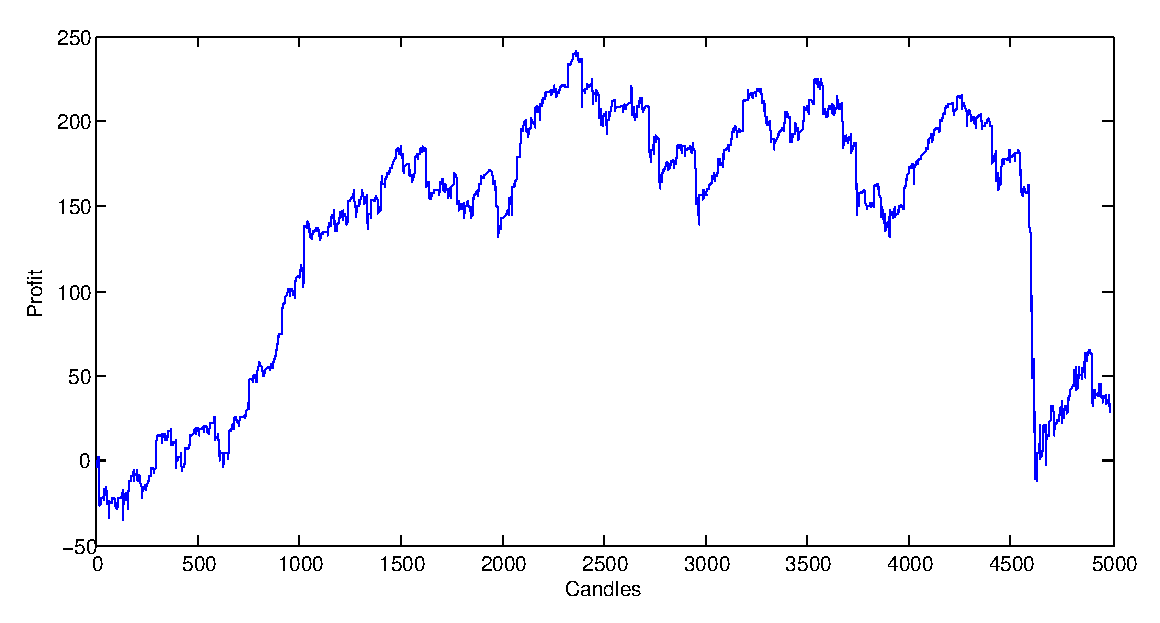
\includegraphics[width=0.82\textwidth]{images/S1c_gold.eps}
\subcaption{Profit- S1c}
\label{cztero}
\end{minipage}
\begin{minipage}{.49\linewidth}
\centering 
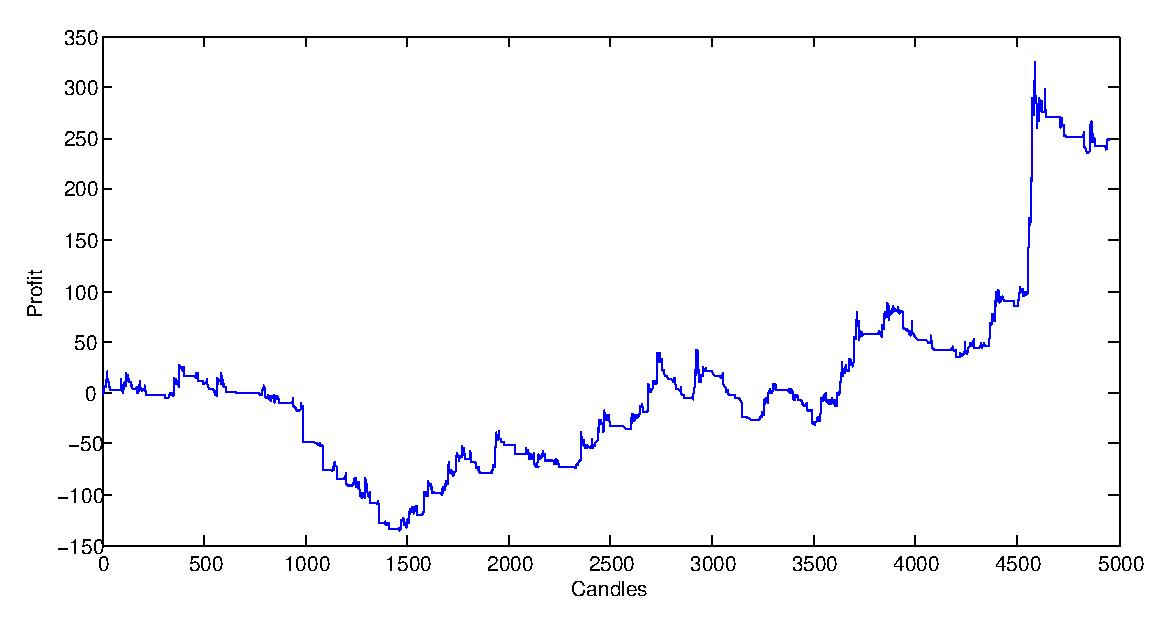
\includegraphics[width=0.82\textwidth]{images/S1d_gold.eps}
\subcaption{Profit - S1d}
\label{mansard}
\end{minipage}
\begin{minipage}{\linewidth}
\centering 
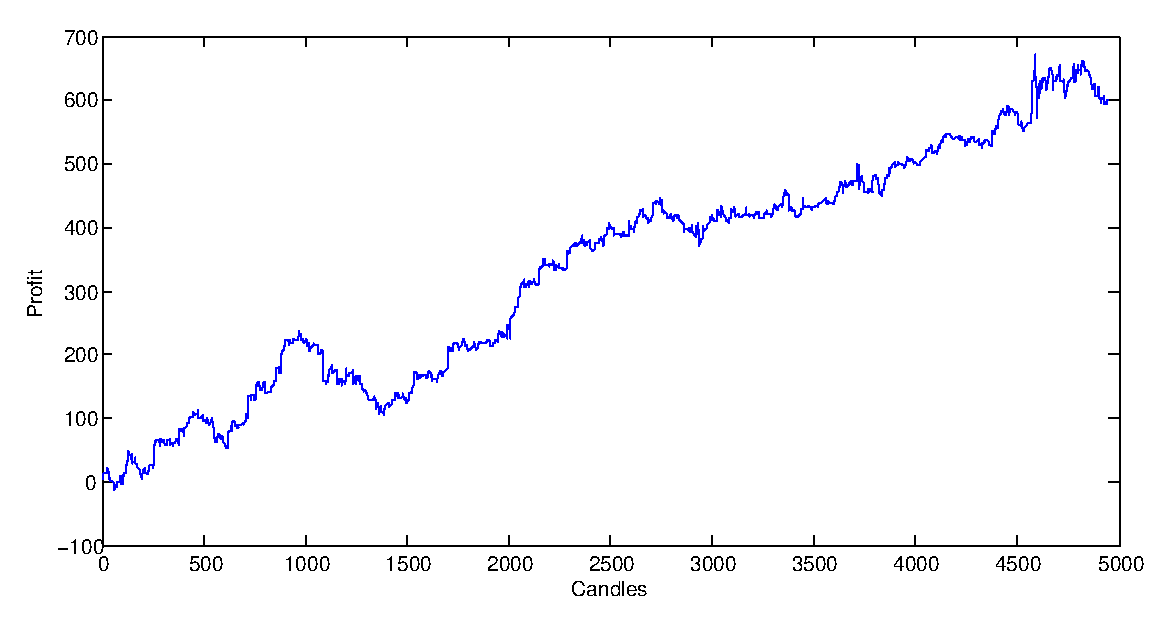
\includegraphics[width=0.6\textwidth]{images/S1s_gold.eps}
\label{mansard}
\subcaption{Profit - S1s}
\end{minipage}
\caption{FGOLD market results}
\end{figure}
\FloatBarrier



%%%%%%%%%%%%%%%%%%%%%%%%%%%%%%%%
\newpage
\begin{table}[!t]
\caption{Profits for all strategy quadrants for FSILVER} 
 \begin{center} 
 \begin{tabular}{|l|l|l|l|l|} 
 \hline \textbf{strategy} & \textbf{profit} & \textbf{bestCalmar} & \textbf{bestMALength} & \textbf{la} \\ \hline  
S1a & -5.31 & -0.65 & 81 & 2582\\ \hline 
S1b & 17.22 & 5.86 & 10 & 2508\\ \hline 
S1c & 4.17 & 0.56 & 10 & 2473\\ \hline 
S1d & 6.95 & 1.33 & 81 & 2336\\ \hline 
S1s & 21.96 & 5.55 & Group of MA & 4918\\ 
\hline \end{tabular} 
 \end{center} 
 \end{table}
\FloatBarrier

\begin{figure}[h]
\centering
\begin{minipage}{.49\linewidth}
\centering 
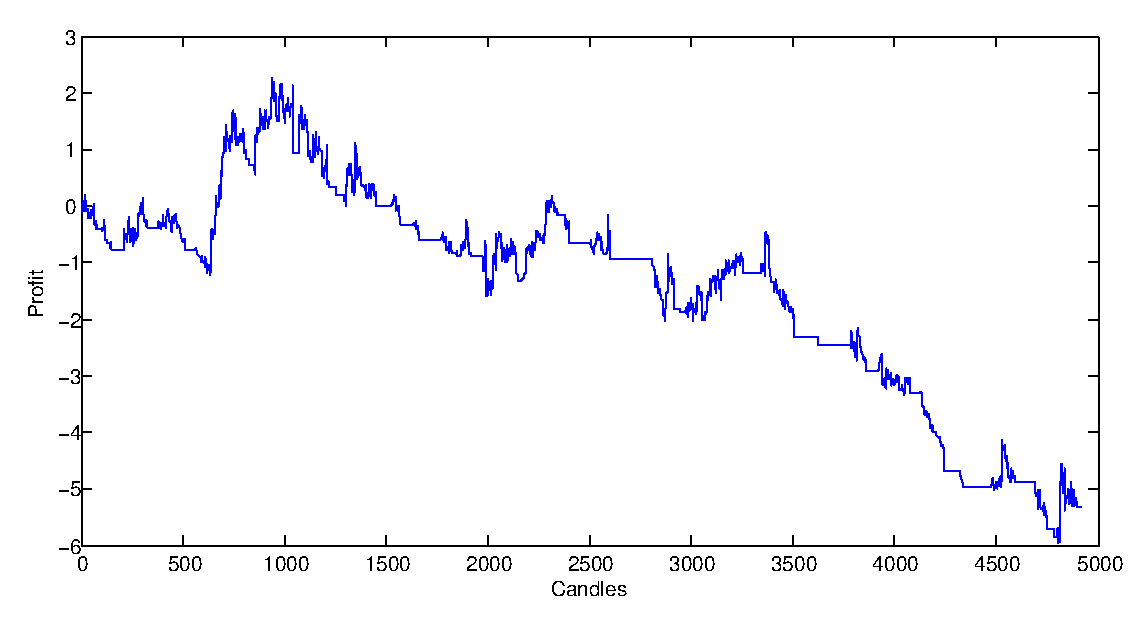
\includegraphics[width=0.82\textwidth]{images/S1a_silver.eps}
\subcaption{Profit - S1a}
\label{jedno}
\end{minipage}
\begin{minipage}{.49\linewidth}
\centering 
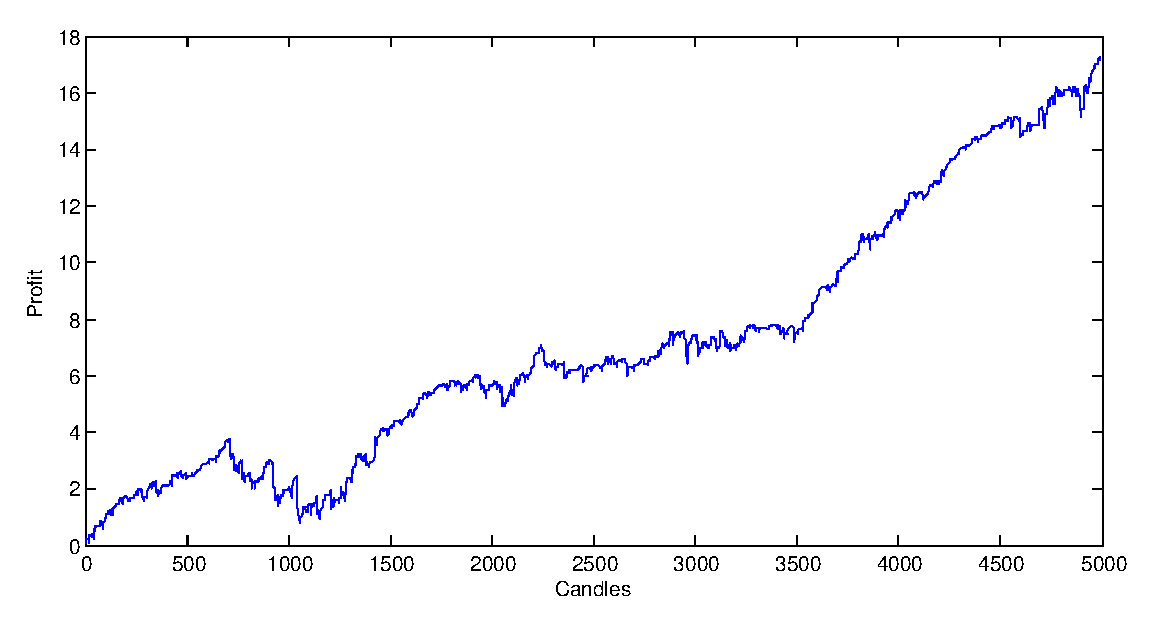
\includegraphics[width=0.82\textwidth]{images/S1b_silver.eps}
\subcaption{Profit - S1b}
\label{dwu}
\end{minipage}
\\
\begin{minipage}{.49\linewidth}
\centering 
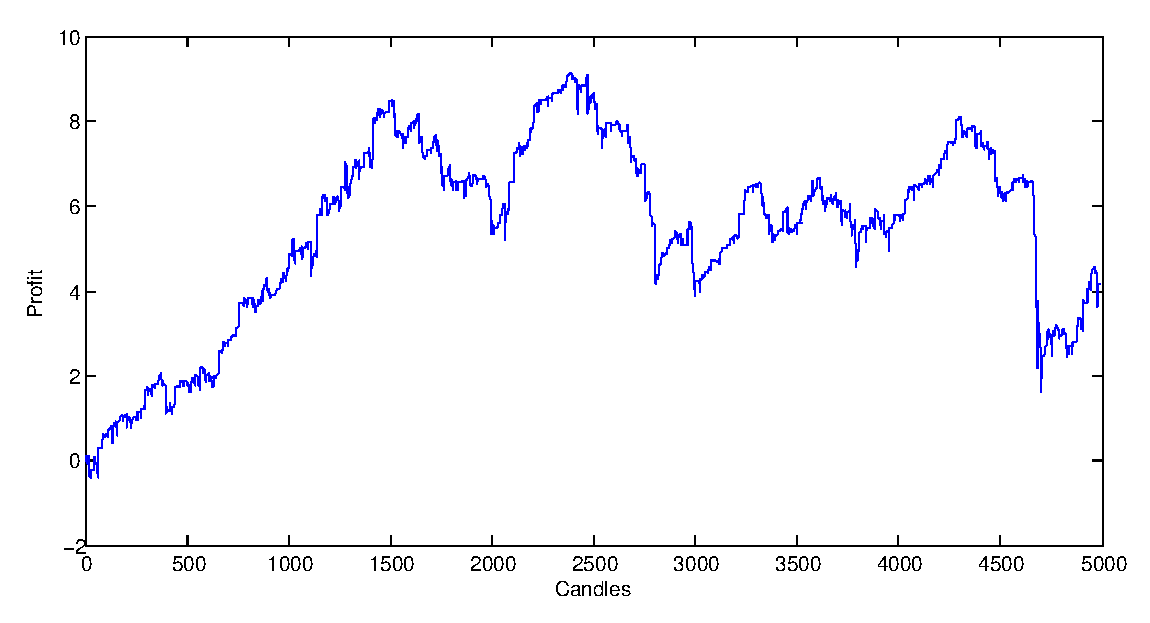
\includegraphics[width=0.82\textwidth]{images/S1c_silver.eps}
\subcaption{Profit- S1c}
\label{cztero}
\end{minipage}
\begin{minipage}{.49\linewidth}
\centering 
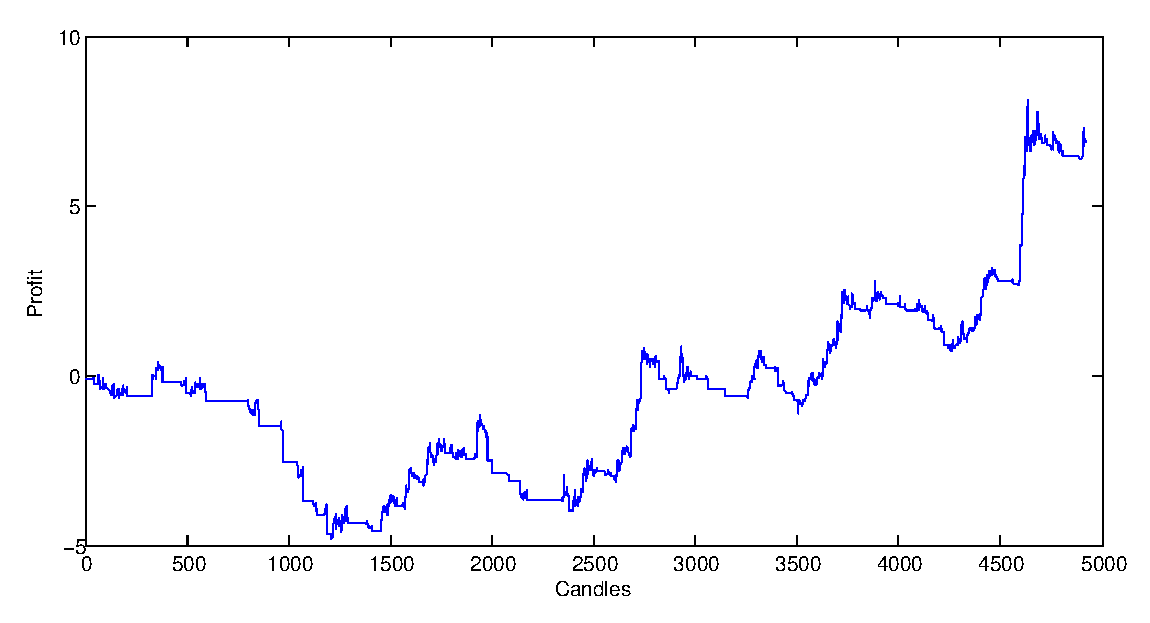
\includegraphics[width=0.82\textwidth]{images/S1d_silver.eps}
\subcaption{Profit - S1d}
\label{mansard}
\end{minipage}
\begin{minipage}{\linewidth}
\centering 
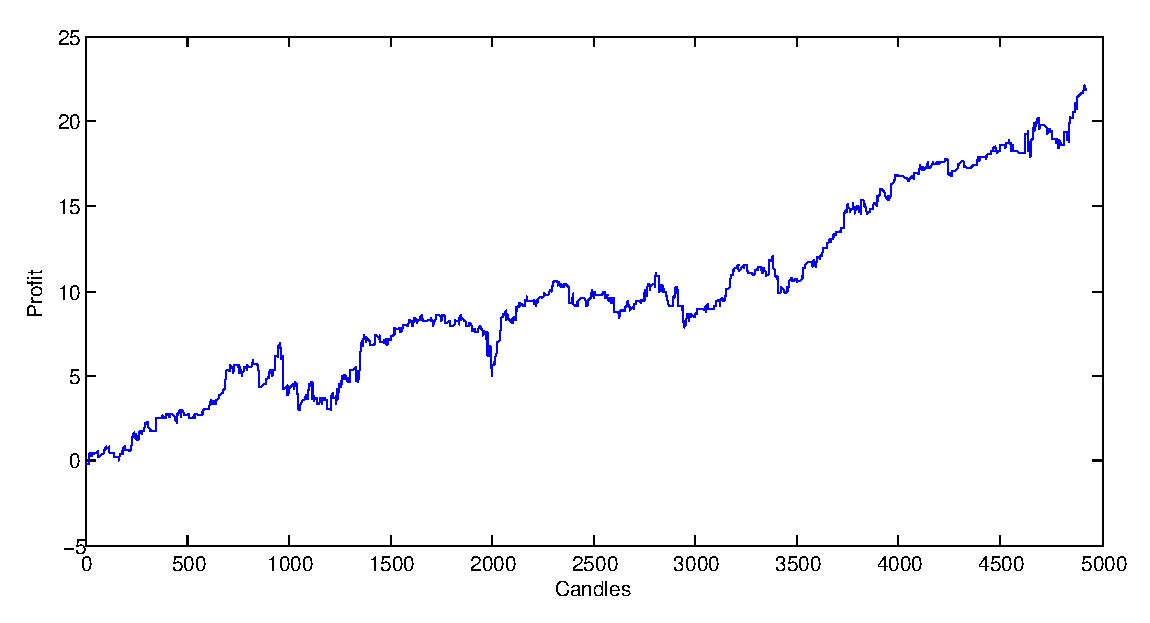
\includegraphics[width=0.6\textwidth]{images/S1s_silver.eps}
\label{mansard}
\subcaption{Profit - S1s}
\end{minipage}
\caption{FSILVER market results}
\end{figure}
\FloatBarrier




%%%%%%%%%%%%%%%%%%%%%%%%%%%%%%%%%%
\section{Conclusions}
\indent Suggested simple strategy is suitable only for algorithmic trading, even in absolute simplest form it seems to be interesting. As it’s been written in the introduction, more from cognitive point of view, than for the transaction value.\\
\indent Surprisingly strategy S1s is a fast and very simple way of receiving really good results, because it is sort of adding each quadrant in one file. In this case results show how surplus grows bigger than loss. \\
\indent This strategy can be modified in many ways.  Eg. in case of suggestions of simultaneous opening long and short positions better is to abandon work than opening both positions (due to transaction costs). The opening of another position in the same direction, eg. long position after closing the previous long position is senseless, it’s better to continue already opened position. These are two simplest ways to improve strategy. There are probably many ways to filter openings that allow to preserve only the most valuable due to profit events. Purpose of this paper was to prove the thesis, that even the simplest strategy has some potential profit, whose using is fascinating challenge.\\
\indent The authors believe, due to observing results of experiments, that the thesis of this dormant potential has been acknowledged. \\
\indent Moreover the results prove that depending on the current market characteristics, it is possible to temporarily disable some quarters from trade in order to getting better profits. Certainly parameters still should be calculated in the background, to be included in trade if market characteristic changes.


%%%%%%%%%% USE ____BIBTEX____ TO GENERATE YOUR REFERENCES 
%%%%%%%%%%% PLEASE UNCOMMENT THE TWO FOLLOWING LINES 

\bibliography{references-tewi}
\bibliographystyle{aiaa-tewi}



\end{document}